\section{Proposed Approach for Topological Validation of Midsurface}

This section presents the approach based on the combinatorial topology~\cite{Hegde2013} for determining the validity of a midsurface computed from CAD model of input sheet metal part. It provides transformation equations based purely on the numbers (that's why the term `combinatorial') of topological entities such as faces, edges, veritces, holes, rings, etc.
%Then count of similar entities in the output shape are predicted based on the transformation equations. Such predicated numbers are matched with the actual numbers in the output shape. Any mismatch hints at the error.
The proposed approach is formulated in two opposite transformation directions, as stated below:

\begin{itemize}
[noitemsep,topsep=2pt,parsep=2pt,partopsep=2pt]
\item \textbf{Solid-to-Surface}: This approach involves predicting output midsurface topological entities using input solid's topological entities.  So, at first, the topological entities of the input solid are counted. The proposed dimension-reduction transformation equations are then applied to predict the topological entities of the corresponding ideal midsurface. These predicted entities are then compared with the actual topological entities of the output midsurface. Any mismatch hints at the error. For example, if the actual number of edges are more than the predicted number of edges, then there is likely gap or missing midsurface patch. Section \ref{sec:topoval:solidsurf} provides more details on this approach. 
%It elaborates on the equations formulated between the topological entities of the input solid and its corresponding midsurface. Apart from matching predicted entities with the actual entities of midsurface, 
In addition, the predicted entities are also checked with standard non-manifold equation (Equation \ref{eqn:topoval:nonmanifold}) to check its validity.% as per theoretical basis of solid modeling.
\item  \textbf{Surface-to-Solid}:  This approach involves predicting the topological entities of the input solid from that of the generated midsurface.  So, at first, the topological entities of the output midsurface are counted. The dimension-addition transformation equations are introduced that are applied to predict the topological entities of the corresponding ideal input solid. These predicted entities of ideal input solid are then compared with the actual topological entities of the input solid.  Any mismatch hints at the error. For example, the predicted entities of solid may not be a closed volume,which ideally should be the case. Section \ref{sec:topoval:surfsolid} provides more details on this approach. 
%It elaborates on  the equations formulated between the topological entities of the output midsurface and its corresponding input solid. Apart from matching predicted with the actual entities of input solid, 
In addition, the predicted entities are also checked with standard manifold equation (Equation \ref{eqn:topoval:manifold}) to check its validity as per theoretical basis of solid modeling.
\end{itemize}

The topological validation method for the midsurface developed in the present research work has been devised for input solids exhibiting sheet metal shape characteristics.
%Section \ref{sec:litsurvey:rscope} elaborates that such thin-walled solids, with constant thickness, pose lesser problems in the computation of the midsurface as well as in the validation of the midsurface, than the ones with variable thickness. 
Although the validation method mentioned here is derived for the constant thickness solids, it can be extended to thin-walled parts with variable thickness as well.
%, e.g., injection-molded plastic parts having drafts. 

%As the proposed approach is based on some of the fundamental concepts of solid modeling, 
The following section gives a brief introduction about some of the fundamental concepts.

\subsection{Theoretical Background}\label{sec:topoval:preliminaries}

Many sheet metal CAD modelers represent thin-walled solid using data structure called a Boundary Representation (Brep). In Brep, a solid is represented by a set of connected faces. This section provides the characteristics of Brep and its classification into manifold and non-manifold representations. In the present research, the term 'manifold' refers to a solid object which is bound, closed and homeomorphic to a topological sphere (also known as 2-manifold), whereas 'non-manifold' object does not have such restrictions to closure and completeness. The present research uses 'non-manifold' mainly to denote surfaces, unless stated otherwise. Another clarification is that, although the term ``surface'' is used while describing transformations from and to solids, the more accurate term is ``face''. Surface is a geometrical entity whereas face is a topological entity. The proposed approach, being related to topology, use of ``surface'' is theoretically incorrect. But as ``midsurface'' is a more widely used term than ``mid-face'', this chapter uses term ``surface'' in place of ``face'' while describing the proposed transformations.

As mentioned in the previous section, the proposed approach provides two transformation equations, one, from input solid to its corresponding midsurface,and the second, from midsurface to its corresponding solid.

Such transformations can be formulated if there is a common topological formulation representing equations for both solids and surfaces. Following subsections present such common formulation.

%%Topological validation devised in this work proposes two transformations with which the quality of a midsurface can be assessed. 
%%
%%\begin{itemize}
%%[noitemsep,topsep=2pt,parsep=2pt,partopsep=2pt]
%%\item \textbf{Solid-to-Surface}: 
%%\item \textbf{Surface-to-Solid}: 
%%\end{itemize}
%%
%%
%%
\subsubsection{Boundary Representation (Brep)}

Brep is composed of two parts: topology and geometry~\cite{Hegde2013}. Topological entities are shells, faces, edges, vertices, etc. whereas geometric entities are surfaces, curves, points, etc. Topological entities are defined as:

\begin{itemize}
[noitemsep,topsep=2pt,parsep=2pt,partopsep=2pt]
\item {\em shell (s)}  is a connected set of {\em faces}
\item {\em face (f)} is a bounded portion of a {\em surface}
\item {\em loop (l)} is a circuit of {\em edges} bounding a {\em face}
\item {\em half-edges (he)} are used to create a {\em loop}.
\item {\em edge (e)} is a bounded portion of a {\em curve}
\item {\em vertex (v)} lies at a {\em point}. 
\end{itemize}

Validity of the Brep model is checked using the Euler-Poincar\'e equation.

\subsubsection{Euler-Poincar\'e Equation}
Euler's equation for polyhedral solids is: \begin{equation}\label{eqn:manifoldsolid}v - e + f = 2\end{equation} where, $v$, $e$, and $f$ represent the number of vertices, edges and faces respectively~\cite{Hegde2013}. It was discovered by Leonhard Euler in 1752 and was later generalized by Lhuilier~\cite{Krishnamurti2002} as follows: \begin{equation}\label{eqn:genmanifoldsolid}v - e + f = 2 - 2g\end{equation} where, $g$ represents genus or holes $h$ or handles ($g$ and $h$ are considered interchangeable in the present research work). Thus, the Euler Poincar\'e equation for manifold-solids is:
%\vspace{-2mm}
\begin{equation}
v - e + (f - r) = 2 (s - h)
\label{eqn:topoval:manifold}
\end{equation} where $r$ represents rings (internal face loop) and $s$ represents shells.

Solids found in the real world have the property that on any point on the boundary, a small enough sphere at that location is split into two pieces, one inside and one outside the object. Non-manifolds do not obey this rule~\cite{Krishnamurti2002}. Weiler (\cite{Weiler1986}) can be attributed for the first significant contribution in defining the non-manifold data structure, called {\em Radial Edge Structure}. Core to this data structure lies the radial cycle, which is an ordered list of faces around an edge.  Similar to manifold, equation for non-manifold topology~\cite{Yamaguchi2002} is: 

\begin{equation}
v - e + (f - r) = s - h
\label{eqn:topoval:nonmanifold}
\end{equation}

Transformation formulation between these two equations, Eqn.~\ref{eqn:topoval:manifold} and Eqn.~\ref{eqn:topoval:nonmanifold}, is apparently not straight-forward. The difference between them is only the constant value $2$ as the multiplier on the right hand sides of Eqn.~\ref{eqn:topoval:manifold}. This constant, which distinguishes between solid and surface is called as a topological invariant, known as Euler's characteristic ($\chi$). 

The significance of this topological invariant is that, for given number of topological entities of a shape, such as faces, edges, vertices, it can predict if the shape is solid or a surface. If it is $2$ it is solid, if it is $1$ it is a surface. Following is an attempt to understand a generic equation encompassing both (solid and surface) dimensionalities in a single equation form.

Brep's topology equation is defined more generically, i.e. for $n$ dimensional object as:

\begin{equation}
\sum_{i=0 }^D(-1)^{i} N_{i}= \sum_{i=0}^D(-1)^{i} \beta_{i} = \chi 
\label{eqn:topoval:betti}
\end{equation}

For dimensions upto 3 ($i=3$), equation (\ref{eqn:topoval:betti}) simplifies to:

\begin{equation}
N_{0}-N_{1}+N_{2}= \beta_{0} -\beta_{1} + \beta_{2}
\label{eqn:topoval:betti3}
\end{equation}

where, $N$s are topological entities of the dimension $0,1$ and $2$ respectively and $\beta$s are the Betti numbers. $\beta_{0}$, $\beta_{1}$ and $\beta_{2}$ correspond to  the number of connected components, holes and cavities, respectively~\cite{Sequin}. One of the fundamental property is that two homeomorphic topological spaces will have the same Euler characteristic and Betti numbers.

\deleted{Most of the CAD models are made up of solids (manifolds), since they are considered to be complete and  having their own volumes. A manifold-solid model can only represent one closed volume minus its internal structure. It cannot represent  heterogeneous possibilities such as wires (curves),  sheets (surfaces),  and  solids (volumes) together, which, although, are not possible in the real world, but are possible during the intermediate stages of design~\cite{Yamaguchi1995}. A non-manifold model is a generic modeling framework which encompasses all these items in a single framework~\cite{Lee2001}.}

The Euler characteristic ($\chi$) in terms of Betti numbers, provides a generic invariant for a shape of any dimension. Manifestation of the Betti numbers in different dimensions is different. So, when input solid is transformed into its corresponding midsurface, the interpretation of the Betti number changes from the manifold domain to the non-manifold domain. Following subsection presents manifestation of the Betti numbers for solids and surfaces respectively, which later will be used to formulate the transformations amongst them.

\subsubsection{Manifold-Solids}

Mapping between topological entities of manifold solids from Euler Poincar\'e Eqn.~\ref{eqn:topoval:manifold} to Betti numbers from Eqn.~\ref{eqn:topoval:betti3} is as follows:

\begin{itemize}
[noitemsep,topsep=2pt,parsep=2pt,partopsep=2pt,label={}]
\item $N_{0} = v $ : number of vertices
\item $N_{1} = e $ : number of edges
\item $N_{2} = (f - r)$ : number of faces ($f$) - additional {\em artifact} edges corresponding to inner loops ($r$)
\item $\beta_{0} = s$ : number of components or disjoint parts ($shells$)
\item $\beta_{1} = 2h$ : number of independent closed curves drawn without splitting. Twice the genus $g$ or $h$. For Torus, there are two such circles and one genus-hole. ($2h$)
\item $\beta_{2} = s$ : number of space regions created by connected surfaces. For an open surface $\beta_{0} = 1$ and $\beta_{2}=0$ whereas for closed surface,  $\beta_{2}$ is equal to $\beta_{0}$,  which is equal to $s$.
\end{itemize}

There is direct mapping between manifold solid's topological entities and Betti numbers. Following subsection investigates if that is true with non-manifold equation as well.

\subsubsection{Non-manifold-Surfaces}


Mapping between topological entities of non manifold surface from Euler Poincar\'e Eqn.~\ref{eqn:topoval:nonmanifold} to Betti numbers from Eqn.~\ref{eqn:topoval:betti3} is as follows:

\begin{itemize}
[noitemsep,topsep=2pt,parsep=2pt,partopsep=2pt,label={}]
\item $N_{0} = v$ : number of vertices
\item $N_{1} = e$ : number of edges
\item $N_{2} = (f - r)$ : number of faces ($f$) -  inner loops ($r$)
\item $\beta_{0} = s$ : number of components or disjoint parts ($shells$)
\item $\beta_{1} = h$ : number of independent closed curves drawn without splitting. Inner holes ( $g$ or $h$). 
\item $\beta_{2} = 0$ : number of space regions created by connected surfaces are not present; so it is $0$.
\end{itemize}

Thus there is direct mapping between non manifold surface's topological entities and Betti numbers. Thus Betti numbers provide equivalence between both, manifold and non-manifold equations, and so, transformations between them is feasible.

\todo{Review comment: Not clear what is th rational of having this section. [ADDED REASON]}

Apart from Brep representing solids, cellular topology has also been used in the present research work (Section~\ref{sec:midsurfcelljoin:fbct}). It has been leveraged in one of the two, transformation directions in the proposed topological validation approach. Following section elaborates its representation and constituents.

\subsubsection{Cellular Topology}
Cellular topology is one of the prominent representations in solid modeling, typically generated by decomposition a solid volume into sub-volumes, called `'cells''. According to Chen et al.~\cite{Chen2006}, a cellular model includes topologies of various dimensions. 
$$\mathbb{M} = 
(\cup_{i=1}^{q} C_i^0 ) \cup 
(\cup_{j=1}^{r} C_j^1 ) \cup  
(\cup_{k=1}^{s} C_k^2 ) \cup 
(\cup_{l=1}^{t} C_l^3 ) $$ where  $C_i^0$ are $0$-dimensional vertices,  $C_j^1$ are $1$-dimensional edges,  $C_k^2$ are $2$-dimensional faces and  $C_l^3$ are $3$-dimensional solids.


Table \ref{tbl:topoval:celldecompexample} shows input solid models along with their corresponding cellular topology models.

%%\bigskip

\begin{minipage}{0.9\linewidth}
%\begin{minipage}{0.9\textwidth} %should be full length even in case of two column
%\resizebox{0.9\linewidth}{!}{
\begin{center}
\captionof{table}{Decomposition of Shapes into Cells}
\label{tbl:topoval:celldecompexample}
\begin{tabular}[h]{@{}p{0.22\linewidth} p{0.22\linewidth}  | p{0.22\linewidth}  p{0.22\linewidth} @{}} \toprule
{\bf Input Solid} & {\bf Cellular Model}  & {\bf Input Solid} & {\bf Cellular Model} \\ \midrule  

\adjustbox{valign=t}{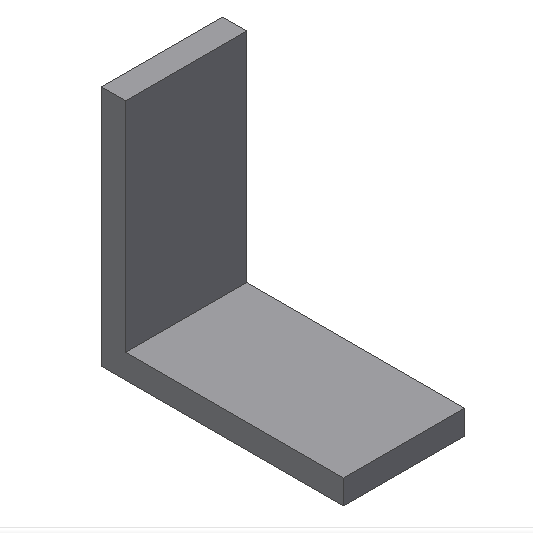
\includegraphics[width=0.8\linewidth]{images/nonCellularL}}  &  
\adjustbox{valign=t}{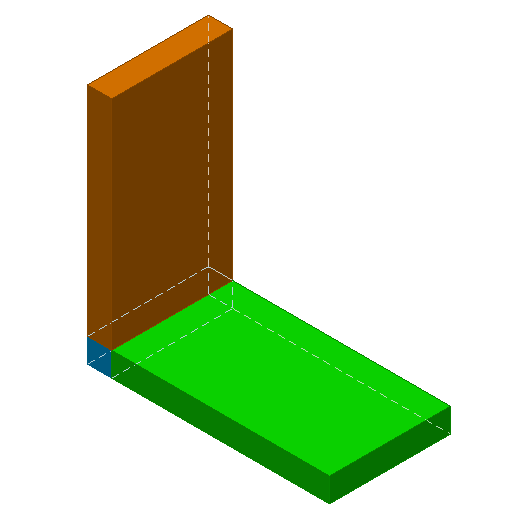
\includegraphics[width=0.8\linewidth]{images/CellularL}}  &

\adjustbox{valign=t}{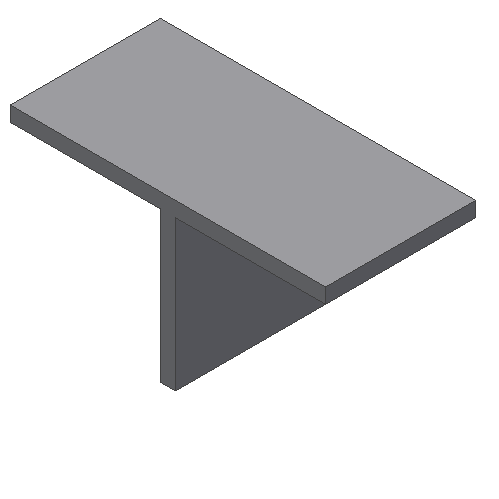
\includegraphics[width=0.8\linewidth]{images/nonCellularT}}  &  
\adjustbox{valign=t}{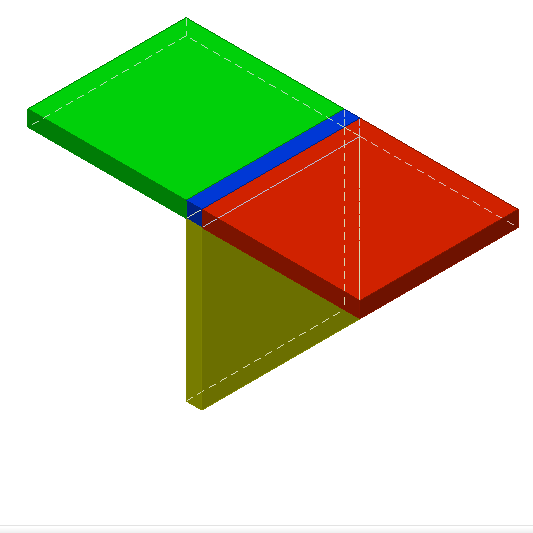
\includegraphics[width=0.8\linewidth]{images/CellularT}} 
\\ \midrule

\adjustbox{valign=t}{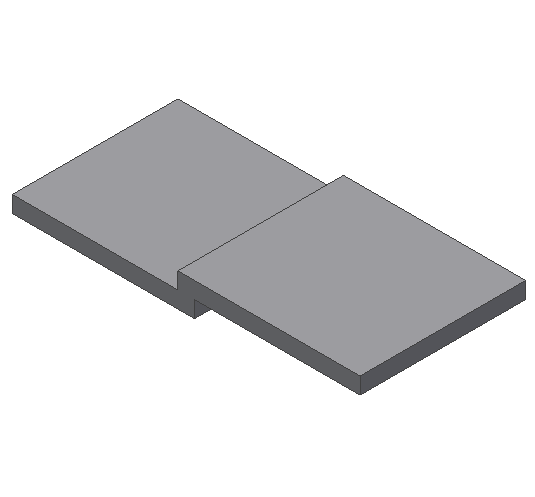
\includegraphics[width=0.8\linewidth]{images/nonCellularOverlap}}  &  
\adjustbox{valign=t}{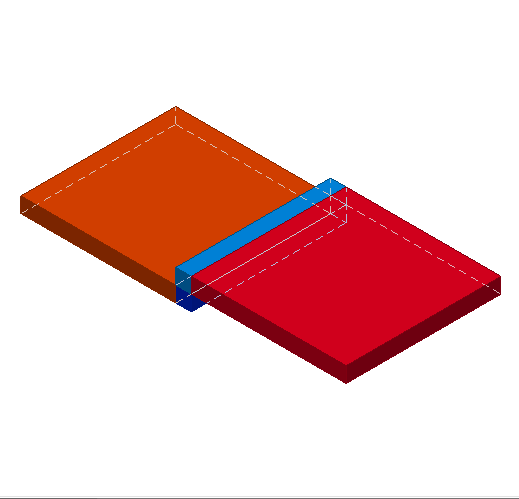
\includegraphics[width=0.8\linewidth]{images/CellularOverlap}}  &

\adjustbox{valign=t}{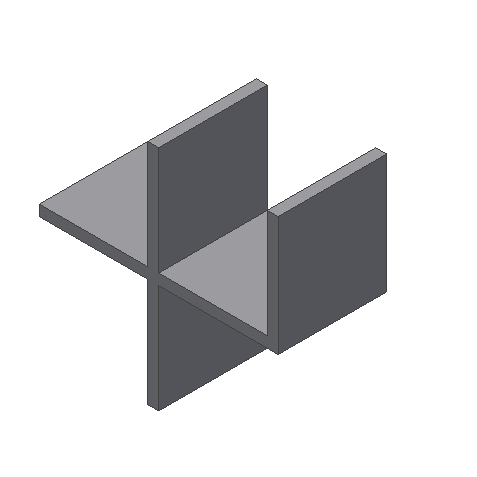
\includegraphics[width=0.8\linewidth]{images/nonCellularZU}}  &  
\adjustbox{valign=t}{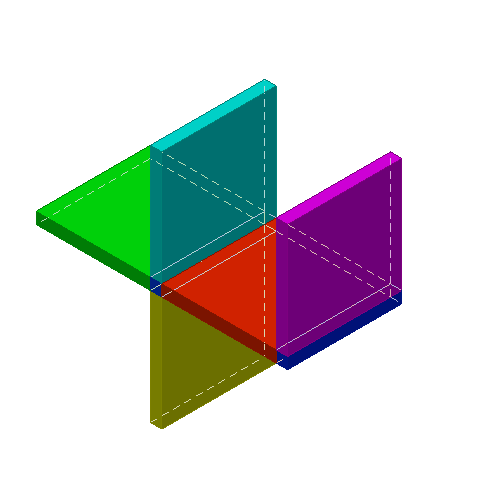
\includegraphics[width=0.8\linewidth]{images/CellularZU}} 
\\ %\midrule

\bottomrule
\end{tabular}

\end{center}
%}
\end{minipage}

\bigskip

The cells have the following properties: 
	\begin{itemize}[noitemsep,topsep=2pt,parsep=2pt,partopsep=2pt]
	\item \textbf{Boundary}: Except $C_i^0$ cells, all cells are bound by cells with a dimension lower by 1.
	\item \textbf{Overlap}: No cells overlap.
	$C_i \cap C_j = \phi$
	\item \textbf{Nature}: Either  additive  or  subtractive.
	\end{itemize}

Following sections elaborate the proposed approach of topological validation, in form of two sub approaches. Both sub-approaches take two inputs viz,  Brep solid of a sheet metal part's CAD model and the Brep midsurface. In the first sub-approach, transformation equation of topological entities between the solid and its corresponding midsurface is derived, whereas in the second, transformation equation of topological entities between the midsurface and its corresponding solid is derived.

%
%%\begin{tabular}[htp]{@{} p{0.4\linewidth} p{0.05\linewidth}  p{0.4\linewidth}@{}} 
%%
%%\adjustbox{valign=t}{
%\begin{minipage}[t]{\linewidth}
%\centering \includegraphics[width=0.2\linewidth]{..//Common/images/Interface2d_1.pdf}
%%\caption{Caption1}
%\captionof{figure}{2D Interface}
%\label{fig:topoval:2dinterface}
%\end{minipage}
%%}
%%
%%&  &
%%
%%\adjustbox{valign=t}{
%\begin{minipage}[t]{\linewidth}
%\centering \includegraphics[width=0.2\linewidth]{..//Common/images/Interface3d_1.pdf}
%%\caption{Caption1}
%\captionof{figure}{3D Interface}
%\label{fig:topoval:3dinterface}
%\end{minipage}
%%} \\
%%
%%\end{tabular}






% ************* OLD FAILED ATTEMPT ********************************
%In the Thin wall manifold solid faces are classified as as $f_p$ (Principal-Main faces) and $f_t$ (Thickness or capping faces). Edges are classified as $e_p$ (Principal-Main edges) and $e_t$ (along thickness or capping edges). Vertices are classified as $v_t$ (thickness vertex) when they are connected to at-least one $e_t$ and $v_p$ (principal or radial vertex), when they are connected to only $e_p$s.
%
%\subsubsection{Steps: Topological dimension reduction}
%\begin{itemize}
%[noitemsep,topsep=2pt,parsep=2pt,partopsep=2pt,leftmargin=*]
%\item Given a manifold solid, half of the $f_p$s are retained in the corresponding midsurface. Thickness faces $f_t$s and edges $e_t$s are gone. 
%%\item {\em Genuses} are the holes and the {\em rings} in the midsurface
%\item Half of the thickness vertices $v_t$s will remain in the midsurface. But the difficulty comes in predicting vertices at the junctions (corresponding to $v_p$s). Additional information about radial group of  $v_p$s is not directly available in the solid model (unless loop traversal detects cycles). 
%\item For example, in case of {\em \bf L} shape, half the $v_p$s are present in the midsurface as radial vertices, but in case of {\em \bf T} shape thats not true. So the procedure which is valid for  junctions up to degree two, is not so for the higher degree junctions. Examples below demonstrate this.
%\item Expand the Solid equation (\ref{eqn:topoval:manifold}) to include newly defined faces, edges: $ (v_p + v_t) - (e_p  + e_t) + (f_p  + f_t) = 2 (s - g) + r$
%\item For midsurface of this Solid, number of topological entities are changed as follows:
%	\begin{itemize}
%	[noitemsep,topsep=2pt,parsep=2pt,partopsep=2pt,label={}, leftmargin=*]
%	\item $v_{nm} = (v_p + v_t)/2$
% 	\item $e_{nm} = e_p/2$
%  	\item $e_t  = f_t  = r = 0$
%  	\item $f_{nm} = f_p/2$
%  	\end{itemize}
%\item Validate if the non-manifold equation $v_{nm} - e+{nm} + f_{nm} == (s_{nm} - g_{nm}) $ is honored.
%\end{itemize}
%
%\subsubsection{Examples}
%\begin{itemize}
%[noitemsep,topsep=2pt,parsep=2pt,partopsep=2pt,leftmargin=*]
%\item For Simple plate:
%	\begin{itemize}
%	[noitemsep,topsep=2pt,parsep=2pt,partopsep=2pt,label={}, leftmargin=*]
%%	\item \textcolor{blue}{``picture of the plate''}
%	\item $f_p =2,f_t=4,e_p=8,e_t=4,v_t=8,v_p=0,s=1,g=0$
% 	\item $v_{nm} = (v_t + v_p)/2 = 8 /2 = 4$
%  	\item $e_{nm} = e_p/2 = 8/2 = 4$
%  	\item $f_{nm} = f_p/2 = 2/2 = 1$
%  	\item $s_{nm} = 1, g_{nm} = 0$
%  	\item $v_{nm} - e_{nm} + f_{nm} = 4 - 4 +1 = 1 = (s_{nm} - g_{nm})$.
%  	\item \textbf{Result}: \textcolor{green}{Valid}
%  	\end{itemize}
%
%\item For 'L' shaped plate:
%	\begin{itemize}
%	[noitemsep,topsep=2pt,parsep=2pt,partopsep=2pt,label={}, leftmargin=*]
%%	\item \textcolor{blue}{``picture of L''}
%	\item $f_p =4,f_t=4,e_p=14,e_t=4,v_t=8,v_p=4,s=1,g=0$
% 	\item $v_{nm} = (v_t + v_p)/2 = (8+4) /2 = 6$
%  	\item $e_{nm} = e_p/2 = 14/2 = 7$
%  	\item $f_{nm} = f_p/2 = 4/2 = 2$
%  	\item $s_{nm} = 1, g_{nm} = 0$
%  	\item $v_{nm} - e_{nm} + f_{nm} = 6 - 7 + 2= 1 = (s_{nm} - g_{nm})$.
%  	\item \textbf{Result}: \textcolor{green}{Valid}
%  	\end{itemize}
%  	
%  	\item For 'T' shaped plate: 
%	\begin{itemize}
%	[noitemsep,topsep=2pt,parsep=2pt,partopsep=2pt,label={}, leftmargin=*]
%%	\item \textcolor{blue}{``picture of T''}
%	\item $f_p =5,f_t=5,e_p=20,e_t=6,v_t=12,v_p=4,s=1,g=0$
% 	\item $v_{nm} = (v_t + v_p)/2 = (12+4) /2 = 8$
%  	\item $e_{nm} = e_p/2 = 20/2 = 10$
%  	\item \textcolor{red}{$f_{nm} = f_p/2 = 5/2 = 2.5$}
%  	\item $s_{nm} = 1, g_{nm} = 0$
%  	\item $v_{nm} - e_{nm} + f_{nm} = 6 - 7 + 2= 1 = (s_{nm} - g_{nm})$.
%  	\item \textbf{Result}: \textcolor{red}{Invalid}
%  	\end{itemize}
%
%\end{itemize}
%
%\textbf{Conclusion}: Manifold equation of Thin Solid cannot be simplistically converted to non-manifold equation of its midsurface. Thus this direction of validation has limitations. Following section examines if the other direction of validation is possible or not.


\subsection{Solid to Midsurface Transformation} \label{sec:topoval:solidsurf}

The approach presented below proposes dimension-reduction-transformation equations for predicting the topological entities of its corresponding midsurface. The solid is first decomposed into ``Cells''. Cells are denoted as $Cell^{dimension}_{attribute}$. The $_{attribute}$ can either be the adjacency information i.e. number of neighbor-touching cells, or can be the type of the cell i.e. $h$ for hole.

Based on the dimensionality of the cells, they are classified as:

\begin{minipage}{0.9\linewidth}
\captionof{table}{Classification of Cells}
\label{tbl:topoval:celltypes}
\begin{tabular}[h]{@{}p{0.1\linewidth}  p{0.1\linewidth}| p{0.4\linewidth} | p{0.35\linewidth}@{}} \toprule
Cell Type & & Description & Topological entities count \\ \midrule
$Cell^3_{*}$  & 
\adjustbox{valign=t}{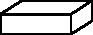
\includegraphics[width=\linewidth]{images/SimplePlate1.pdf}} &
3D cells (solids), topologically similar to a simple plate &
 $faces=6 \newline edges=12 \newline vertices =8$ \\
 
 $Cell^{2}_{*}$ &
 \adjustbox{valign=t}{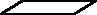
\includegraphics[width=\linewidth]{images/SimplePlane1.pdf}} &
  2D cells, topologically similar to a planar surface  &
   $faces=1 \newline edges=4 \newline vertices =4$ \\
   
$Cell^{1}_{*}$ &
 \adjustbox{valign=t}{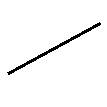
\includegraphics[width=\linewidth]{images/SimpleLine1.pdf}} &
1D cells, topologically equivalent to a line &
 $edges=1  \newline vertices =2$ \\
 
 $Cell^{2}_{h}$ &
  \adjustbox{valign=t}{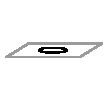
\includegraphics[width=\linewidth]{images/SimpleHole1.pdf}} &
  Hole is assumed to be cylindrical through-all (true for sheet metal parts) &
   $edges=1  \newline vertices =1$ \\ \bottomrule
 \end{tabular}

\end{minipage}

\bigskip

Table~\ref{tbl:topoval:celltypes} shows various cell types along with the count of their topological entities. These counts are their contribution to the overall count of topological entities in the formulation developed below. First row shows a 3D cell, of a shape like a plate. Thus it has 6 $faces$, 12 $edges$ and 8 $vertices$. The second row, shows a 2D cell, represents rectangular faces, has 1 $face$, 4 $edges$ and 4 $vertices$. Similarly other cell types are defined.

The cells are then classified into $sCell$s and $iCell$s as per definitions \ref{def:midsurfcelljoin:scell} and \ref{def:midsurfcelljoin:icell}, respectively. The midsurface cell is of dimension two, so it is represented as $mCell^2$. Figure~\ref{fig:topoval:treekexample} shows ``L'' shaped solid being decomposed into  3 cells, two of which are $sCell$s and one is $iCell$.

\begin{figure}[!h]
\centering     %%% not \center
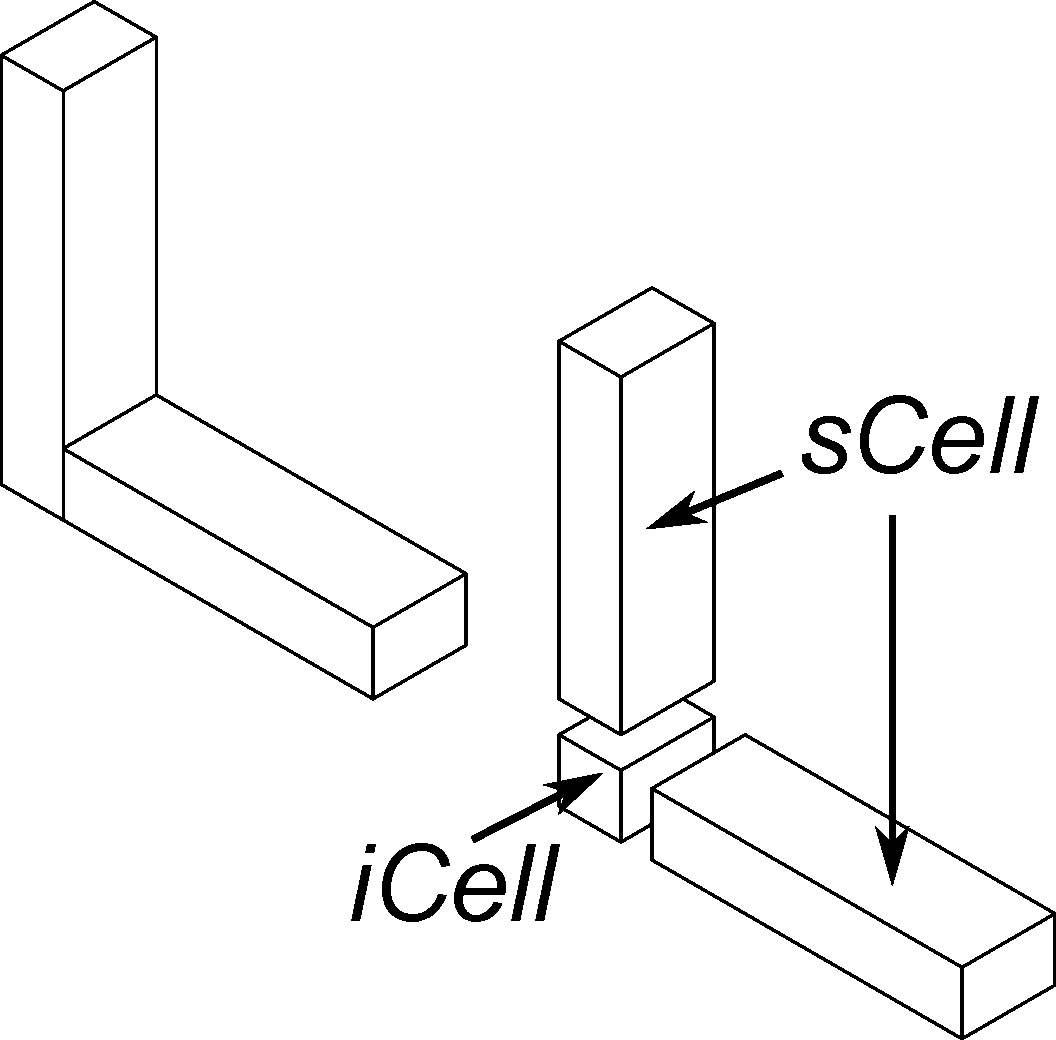
\includegraphics[width=0.25\linewidth]{images/CellDecompExample.pdf}
\caption{Decomposition and Classification of Cells}
%\caption{Decomposition and Classification of Cells (Source: Treeck \cite{Treeck})}
\label{fig:topoval:treekexample}
\end{figure}


$iCell$s can be surface interfaces or 2D interfaces, denoted by $iCell^2$ and solid interfaces or 3D interfaces, denoted as $iCell^3$. Figure~\ref{fig:topoval:interfacetypes}a shows surface touching of two solid cells, also known as `face overlap' and  Figure~\ref{fig:topoval:interfacetypes}b shows volumetric overlap, which after cellular decomposition generates 3D interface cell.

	\begin{figure}[!h]
	\centering     %%% not \center
	\subfloat[Face Overlap]{\label{fig:topoval:2dinterface}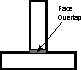
\includegraphics[width=0.25\linewidth,valign=t]{images/Interface2d_2.pdf}} \qquad
	\subfloat[Volume Overlap]{\label{fig:topoval:3dinterface}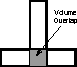
\includegraphics[width=0.25\linewidth,valign=t]{images/Interface3d_2.pdf}}
	\caption{Face and Volume Interactions of Cells}
	\label{fig:topoval:interfacetypes}
	\end{figure}



%%\begin{tabular}[htp]{@{} p{0.3\linewidth} p{0.05\linewidth}  p{0.55\linewidth}@{}} 
%
%
%%&&
%
%%\adjustbox{valign=t}{
%\begin{minipage}[t]{\linewidth}
%\centering 
%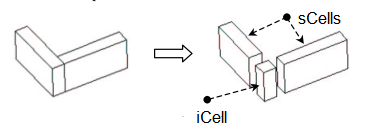
\includegraphics[width=0.6\linewidth]{images/CellDecompExample}
%%\vspace{\abovecaptionskip}
%\captionof{figure}{Decomposition \& classification\cite{Treeck}}
%\label{fig:topoval:treekexample}
%\end{minipage}
%%}		
%%\\
%%\end{tabular}

%
%
%
%
%
%\begin{itemize}[noitemsep,topsep=2pt,parsep=2pt,partopsep=2pt]
%\item Two cells touching each other with an area-overlap, is called 2d-Interface.
%\item Two cells touching each other with a volume-overlap, is called 3d-Interface.
%\end{itemize}
	
%If two bodies spatially overlap then they are split to form the 3D interface  (Fig. ~\ref{fig:topoval:3dinterface})  cell. In case of 2D Interface (Fig. ~\ref{fig:topoval:2dinterface}), adjoining faces of the overlapping face is extended \cite{Woo2002} and used as a  cutting tool to create the intersecting volume, the 3D Interface (Fig. ~\ref{fig:topoval:3dinterface}) cell.
%
%	\begin{figure}[!h]
%	\centering     %%% not \center
%	\subfloat[2D Interface]{\label{fig:topoval:2dinterface}\includegraphics[width=0.25\linewidth,valign=t]{images/Interface2d_1.pdf}}
%	\subfloat[3D Interface]{\label{fig:topoval:3dinterface}\includegraphics[width=0.25\linewidth,valign=t]{images/Interface3d_1.pdf}}
%	\caption{2D and 3D Interfaces}
%	\label{fig:topoval:interfacetypes}
%	\end{figure}
%Prefix $s$ is applied if the $Cell$ is from the input shape, $i$ if it is of a newly-introduced interface type,(Fig.~\ref{fig:topoval:treekexample}) and $m$ for midsurface cells.
% Definitions \ref{def:midsurfcelljoin:scell} and \ref{def:midsurfcelljoin:icell}).% Topology generated by the volumetric decomposition is called {\em Cellular Topology}. 

%
%Many commercial as well as academic methods are available for cellular-volumetric decomposition \cite{Woo2002, Chong2004, Cao2011,  Boussuge2013, Kim2014}. 
%Woo (maximal cells \cite{Woo2003}), Boussuge (Extrusion decomposition \cite{Boussuge2013a}), Wu (Sweep Decomposition \cite{Wu2014}), Woo (Protrusion decomposition \cite{Woo2014}), etc. are some of the known cellular decomposition methods used for feature recognition (FR).
%
%Cellular decomposition starts facing problems as the complexity of the original solid increases. The method becomes very slow as the number of cells increases \cite{Woo2003}. If the cutting faces are extended infinitely and intersected with the whole solid then they generate a large number of unnecessary cells. If the splits are not clean, it may generate degenerate entities such as edges and vertices. The topological validation method presented here assumes `clean' cellular decomposition and if it is not so, then the validation results could be unpredictable.


%\begin{center}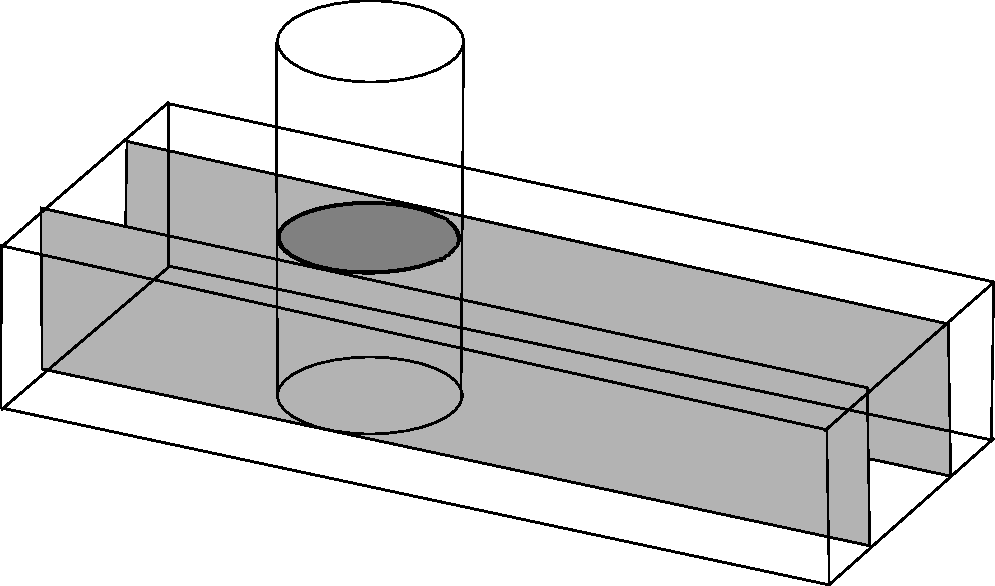
\includegraphics[width=0.6\linewidth]{images/VolDecomp.pdf}\end{center}
%\vspace{-0.8cm}
%\begin{center}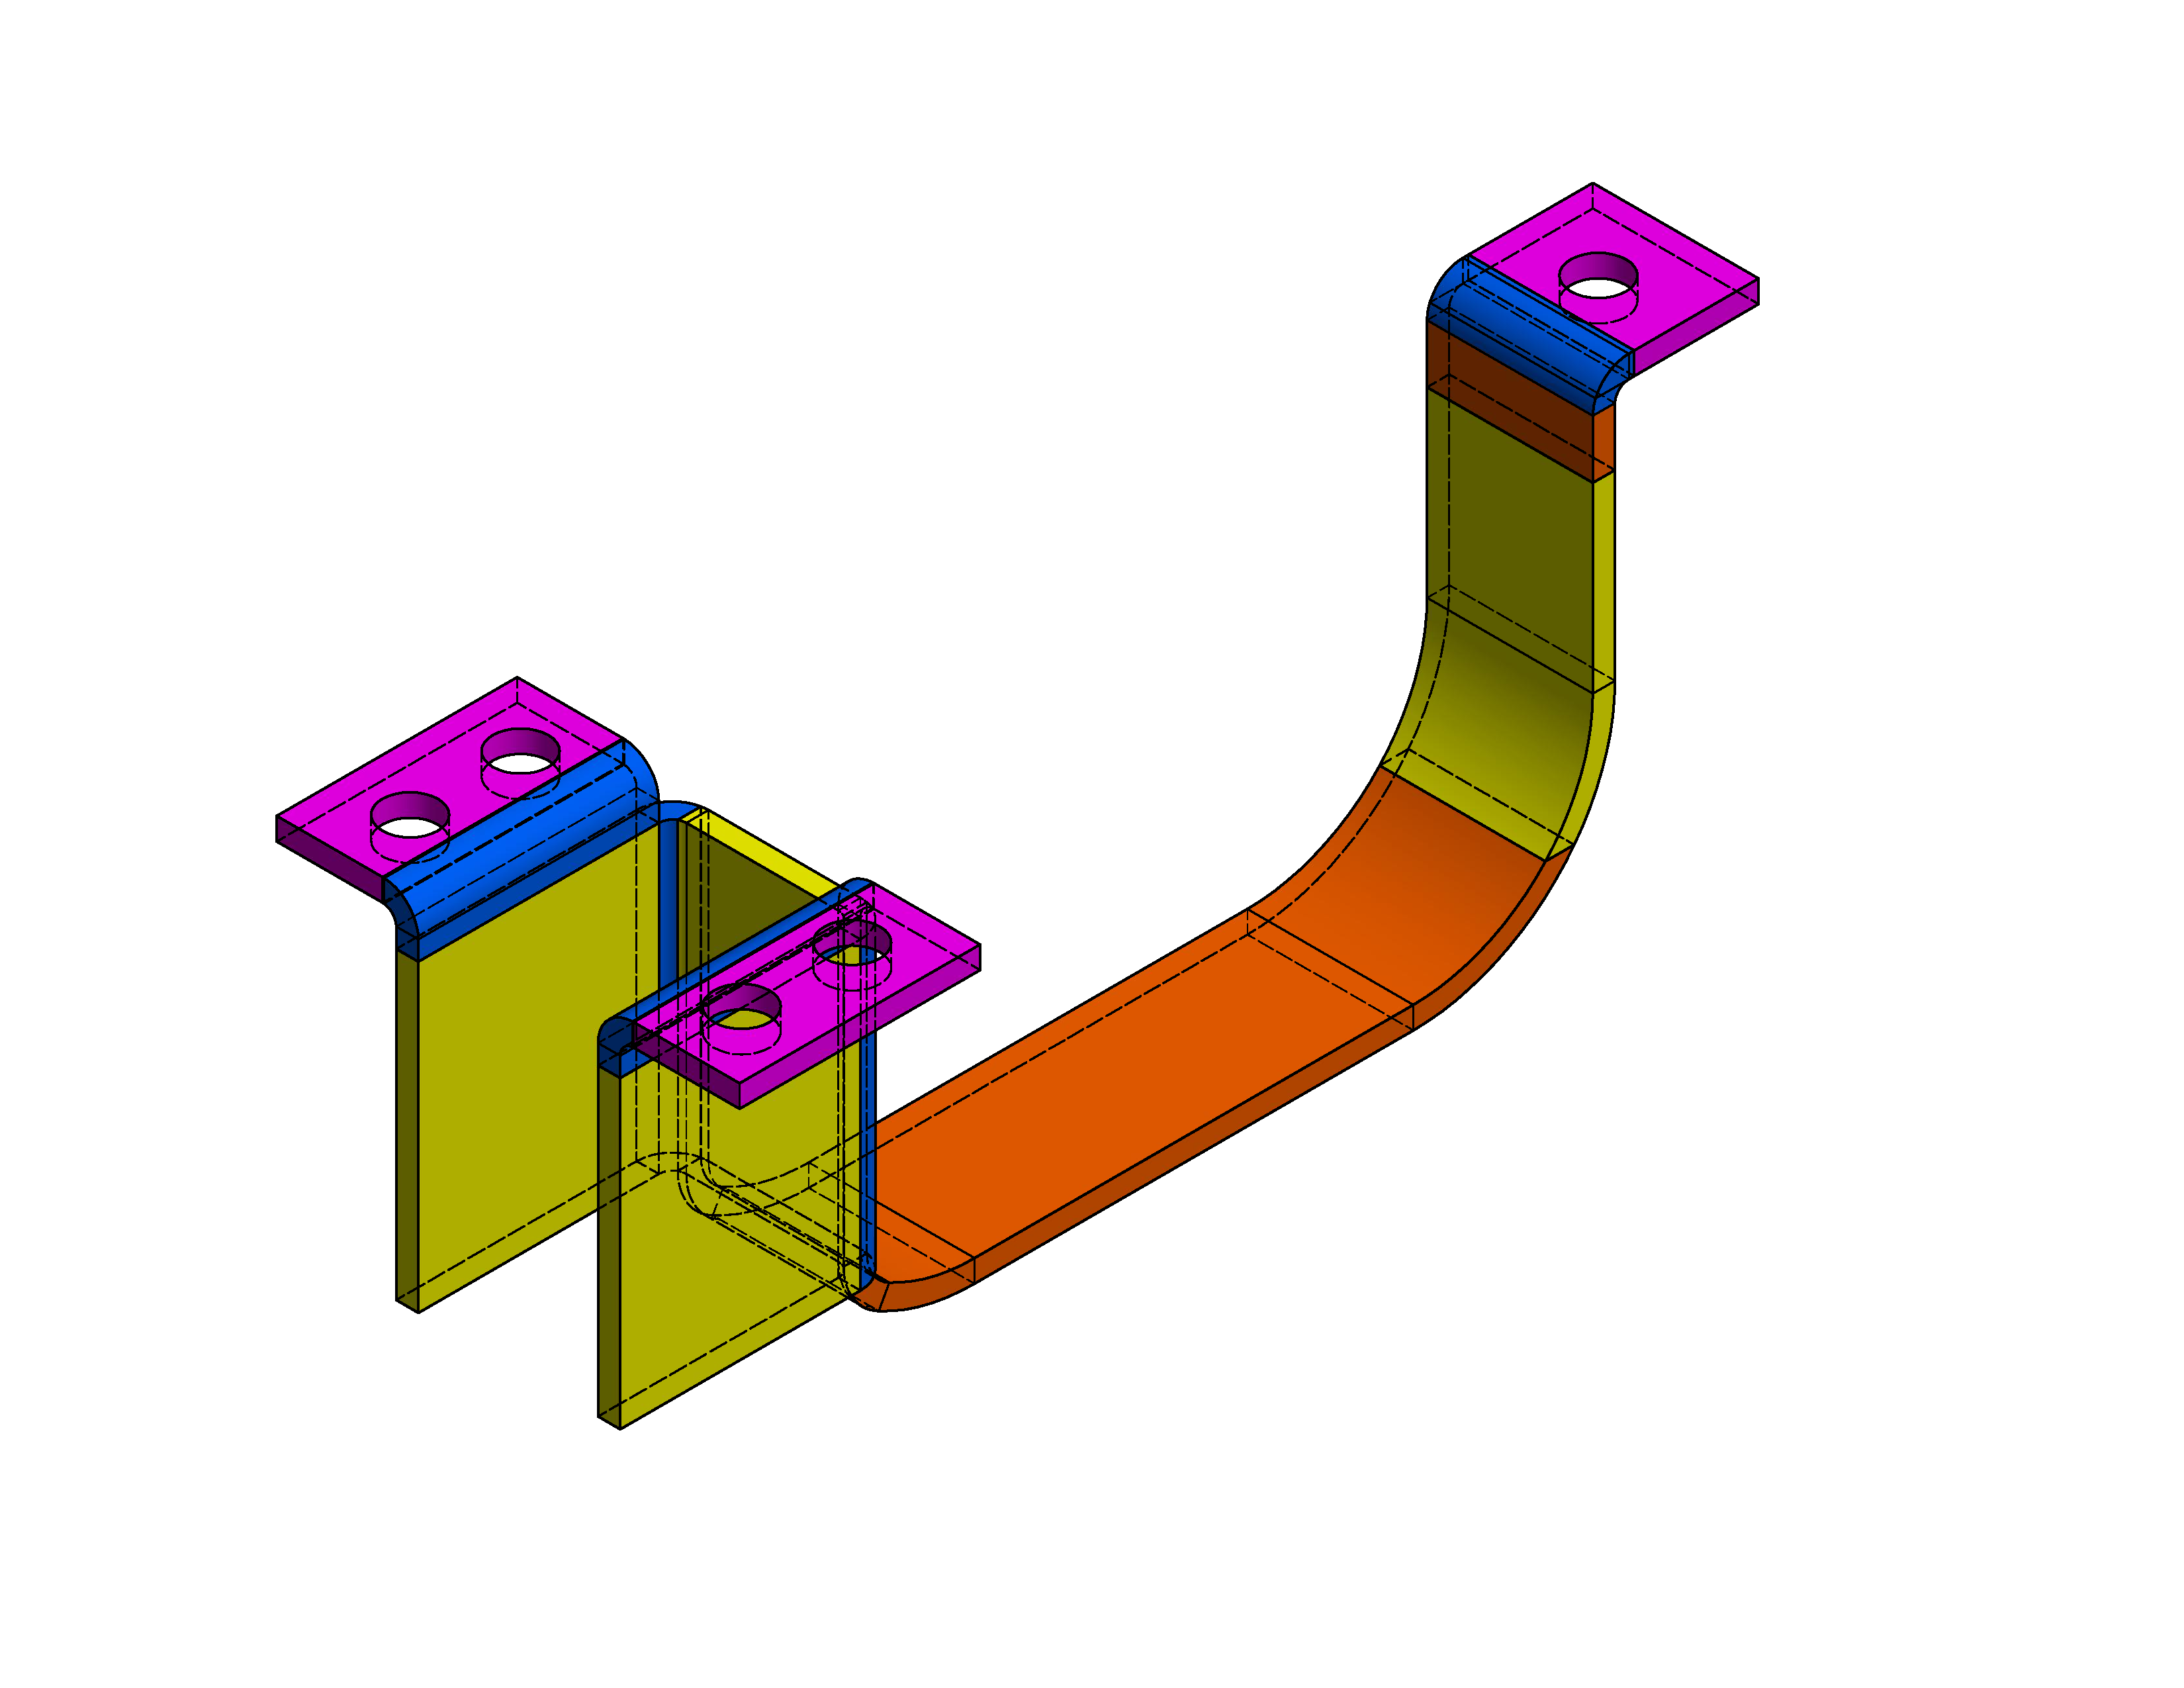
\includegraphics[width=0.6\linewidth]{images/VolDecomp1.pdf}\end{center}
%\vspace{-1.2cm}

%\subsubsection{Steps: Topological Dimension Reduction}
Topological transformation of solid (3D cells) to its corresponding midsurface (2D cells) is as follows:

\begin{itemize}
[noitemsep,topsep=2pt,parsep=2pt,partopsep=2pt]

	\item  $sCell^{3}_{n}$: Solid cell with $adjacency = n$, i.e. $n$ touching sides, transforms into midsurface cell $mCell^2_{n}$, a surface having $n$ edges. Its topological entities are predicted by following equations as:
	
\begin{align}
f=1;
e=4-n;
v=4-2n
\label{eqn:topoval:cellularna}
\end{align} 

\todo{Review comment: without figure it is difficult to imagine. [ADDED FIGURE]}

	\begin{figure}[!h]
	\centering     %%% not \center
	\subfloat[$sCell^{3}_{n}$]{\label{fig:topoval:2sCell}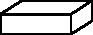
\includegraphics[width=0.25\linewidth,valign=t]{images/SimplePlate1.pdf}} \qquad
	\subfloat[ $mCell^2_{n}$]{\label{fig:topoval:3mCell}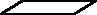
\includegraphics[width=0.25\linewidth,valign=t]{images/SimplePlane1.pdf}}
	\caption{Transformation of Solid Cell to Its Midsurface }
	\label{fig:topoval:s3m2}
	\end{figure}
	
Figure~\ref{fig:topoval:s3m2} shows a simple plate shaped $sCell$ to explain the transformation. This $sCell$ has 6 faces, 12 edges and 8 vertices. It is connected with other $n$ cells. When this cell gets transformed to midsurface patch $mCell^2$ then it has entities given by Eq. ~\ref{eqn:topoval:cellularna}. First row of Table~\ref{tbl:topoval:simpleshapes1} shows the same case, predicting midsurface entities with $n=0$, as no other cells are touching this $sCell$.

	\item   $sCell^{3}_{h}$ : $_h$ denotes `hole' i.e. a negative solid cell representing. It transforms into midsurface cell  $mCell^{2}_{h}$, a hole in the surface. Its topological entities are predicted as:
\begin{equation}
e=1; v=1
\label{eqn:topoval:cellularah}
\end{equation} 

	\item $iCell^{3}_{n}$ : Interface solid cell with $n$ adjacent touching sides transforms into midsurface cell  $mCell_{1,n}$, a edge. Its topological entities are predicted as:

\begin{equation}
e=1;
v=2
\label{eqn:topoval:cellulara}
\end{equation}

Second row of Table~\ref{tbl:topoval:simpleshapes1}, i.e. ``L'' case, has 3 cells, 2 $sCell^{3}_{0}$s and one $ iCell^{3}_{2}$. For the interface cell $ iCell^{3}_{2}$, $n=2$, as it is touching 2 solid cells. It will get transformed into an edge with predicted entities as per Eq.~\ref{eqn:topoval:cellulara}.

	\item  $iCell^{2}_{2}$ :	Interface face cell touched from both sides  transforms into midsurface cell  $mCell^{1}_{2}$, a edge. Its topological entities are predicted as:
\begin{equation}
e=1;
v=2
\label{eqn:topoval:cellularaf}
\end{equation}


\end{itemize}

%(Eqn   \ref{eqn:topoval:cellulara}, \ref{eqn:topoval:cellularaf}, \ref{eqn:topoval:cellularna}, \ref{eqn:topoval:cellularah} )

%\subsubsection{Examples}
Table~\ref{tbl:topoval:simpleshapes1} lists various basic shapes and their dimension-reduction-transformations into their corresponding midsurface
%It is evident that the predicted midsurface entities of these simple shapes match with the actual ones, thus the derived formulation works for these simple shapes. 


%%\bigskip

%\begin{minipage}{\linewidth}
\begin{minipage}{\linewidth}
\begin{center}
\captionof{table}{Topological Validation of Midsurface by Dimensional Reduction}
\label{tbl:topoval:simpleshapes1}
\begin{tabular}[t]{@{}p{0.1\linewidth} p{0.14\linewidth} | p{0.15\linewidth} |  p{0.15\linewidth} | p{0.33\linewidth}@{}}  \toprule

%\captionof{table}{Topological Validation of Midsurface by Dimensional Reduction}
%\begin{longtable}[h]{@{}p{0.1\linewidth} p{0.14\linewidth} | p{0.15\linewidth} |  p{0.15\linewidth} | p{0.33\linewidth}@{}}  \toprule
%\caption{Topological Validation of Midsurface by Dimensional Reduction}
{\bf Solid} & {\bf Midsurface}  & {\bf Solid Cells} & {\bf Midsurface Cells}  & {\bf Predicted Topological Entities} \\ \midrule  

\adjustbox{valign=c}{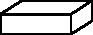
\includegraphics[width=\linewidth]{images/SimplePlate1.pdf}}  &  
\adjustbox{valign=c}{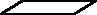
\includegraphics[width=\linewidth]{images/SimplePlane1.pdf}} &  
$sCell^{3}_{0}$ & $ mCell^{2}_{0}$ & 
$ 1f+(4-0)e+(4- 2\times 0)v \newline = 1f+4e+4v$
\\ %\midrule

\adjustbox{valign=c}{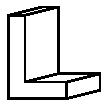
\includegraphics[width=\linewidth]{images/LPlate1.pdf}}  &  
\adjustbox{valign=c}{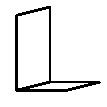
\includegraphics[width=\linewidth]{images/LPlane1.pdf}} &  

$2 \times sCell^{3}_{1} \newline + iCell^{3}_{2}$ & $2 \times mCell^{2}_{1} \newline + mCell^{1}_{2}$  & 
$ 2 \times (1f + (4-1)e+(4-2\times 1)v ) \newline + (1e + 2v) \newline = 2f+7e+6v$ 
\\ %\midrule


\adjustbox{valign=c}{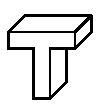
\includegraphics[width=\linewidth]{images/TPlate1.pdf}}  &  
\adjustbox{valign=c}{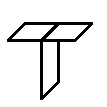
\includegraphics[width=\linewidth]{images/TPlane1.pdf}} &  

$3 \times sCell^{3}_{1} + iCell^{3}_{3}$   &  $3 \times mCell^{2}_{1}  + mCell^{1}_{3}$  & 
$3 \times (1f+(4-1)e+ (4-2\times 1)v)  + (1e+2v)  = 3f+10e+8v$ 
\\ %\midrule

\adjustbox{valign=c}{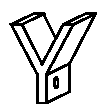
\includegraphics[width=\linewidth]{images/YwithHole1.pdf}}  &  
\adjustbox{valign=c}{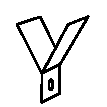
\includegraphics[width=\linewidth]{images/YwithHolem1.pdf}} &  

$3 \times sCell^{3}_{1}  + iCell^{3}_{3}  + sCell^{3}_{h}$   &  
$3 \times mCell^{2}_{1}  + mCell^{1}_{3}  + mCell^{2}_{h}$  & 
$3 \times (1f+(4-1)e+ (4-2\times 1)v)  + (1e+2v)  + (1e+1v)  = 3f+11e+9v$
\\ %\midrule

\adjustbox{valign=c}{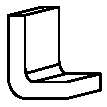
\includegraphics[width=\linewidth]{images/LwithRound1.pdf}}  &  
\adjustbox{valign=c}{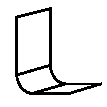
\includegraphics[width=\linewidth]{images/LwithRoundm1.pdf}} &  

$2 \times sCell^{3}_{1}  + 2 \times  iCell^{2}_{2}  + sCell^{3}_{2}$   &  
$2 \times mCell^{2}_{1}  + 2 \times mCell^{1}_{2}  + mCell^{2}_{2}$  & 
$2 \times (1f+(4-1)e+ (4-2\times 1)v)  + 2 \times (1e+2v)  + (1f+(4-2)e+ (4-2\times 2)v)  = 3f+10e+8v$
\\ 

\bottomrule
%
%\label{tbl:topoval:simpleshapes1}
%
%\end{longtable}
%\end{center}
\end{tabular}


\end{center}
\end{minipage}

%%\bigskip

One sample case is explained here. The third row, case ``T'', shows solid model and corresponding midsurface in first two columns. Cellular decomposition of the solid results in 3 solid cells  $sCell^{3}_{1}$, each with $n=1$, i.e. 1 adjacent cell and one interface cell  $iCell^{3}_{3}$. So the solid is represented $3 \times sCell^{3}_{1} + iCell^{3}_{3}$. Dimension reduction of these cell, reduces the dimensionality by 1, and thus result in midsurface equation $2 \times mCell^{2}_{1} \newline + mCell^{1}_{2}$. Each of these transformations contribute topological entities as per Eqn.~\ref{eqn:topoval:cellularna} and Eqn.~\ref{eqn:topoval:cellulara}, and result in predicted midsurface entities as $3 \times (1f+(4-1)e+ (4-2\times 1)v)  + (1e+2v)  = 3f+10e+8v$ i.e. 3 faces, 10 edges and 8 vertices.
%\end{center}
%\end{minipage}

Figure~\ref{fig:midsurfcelljoin:solidsurfbracket} shows working of the above mentioned approach on a relatively-complex practical shape.  

%%\bigskip

\begin{figure}[h!]
\centering     %%% not \center
\subfloat[Input Solid Model]{\label{fig_SimpleBracketshaded}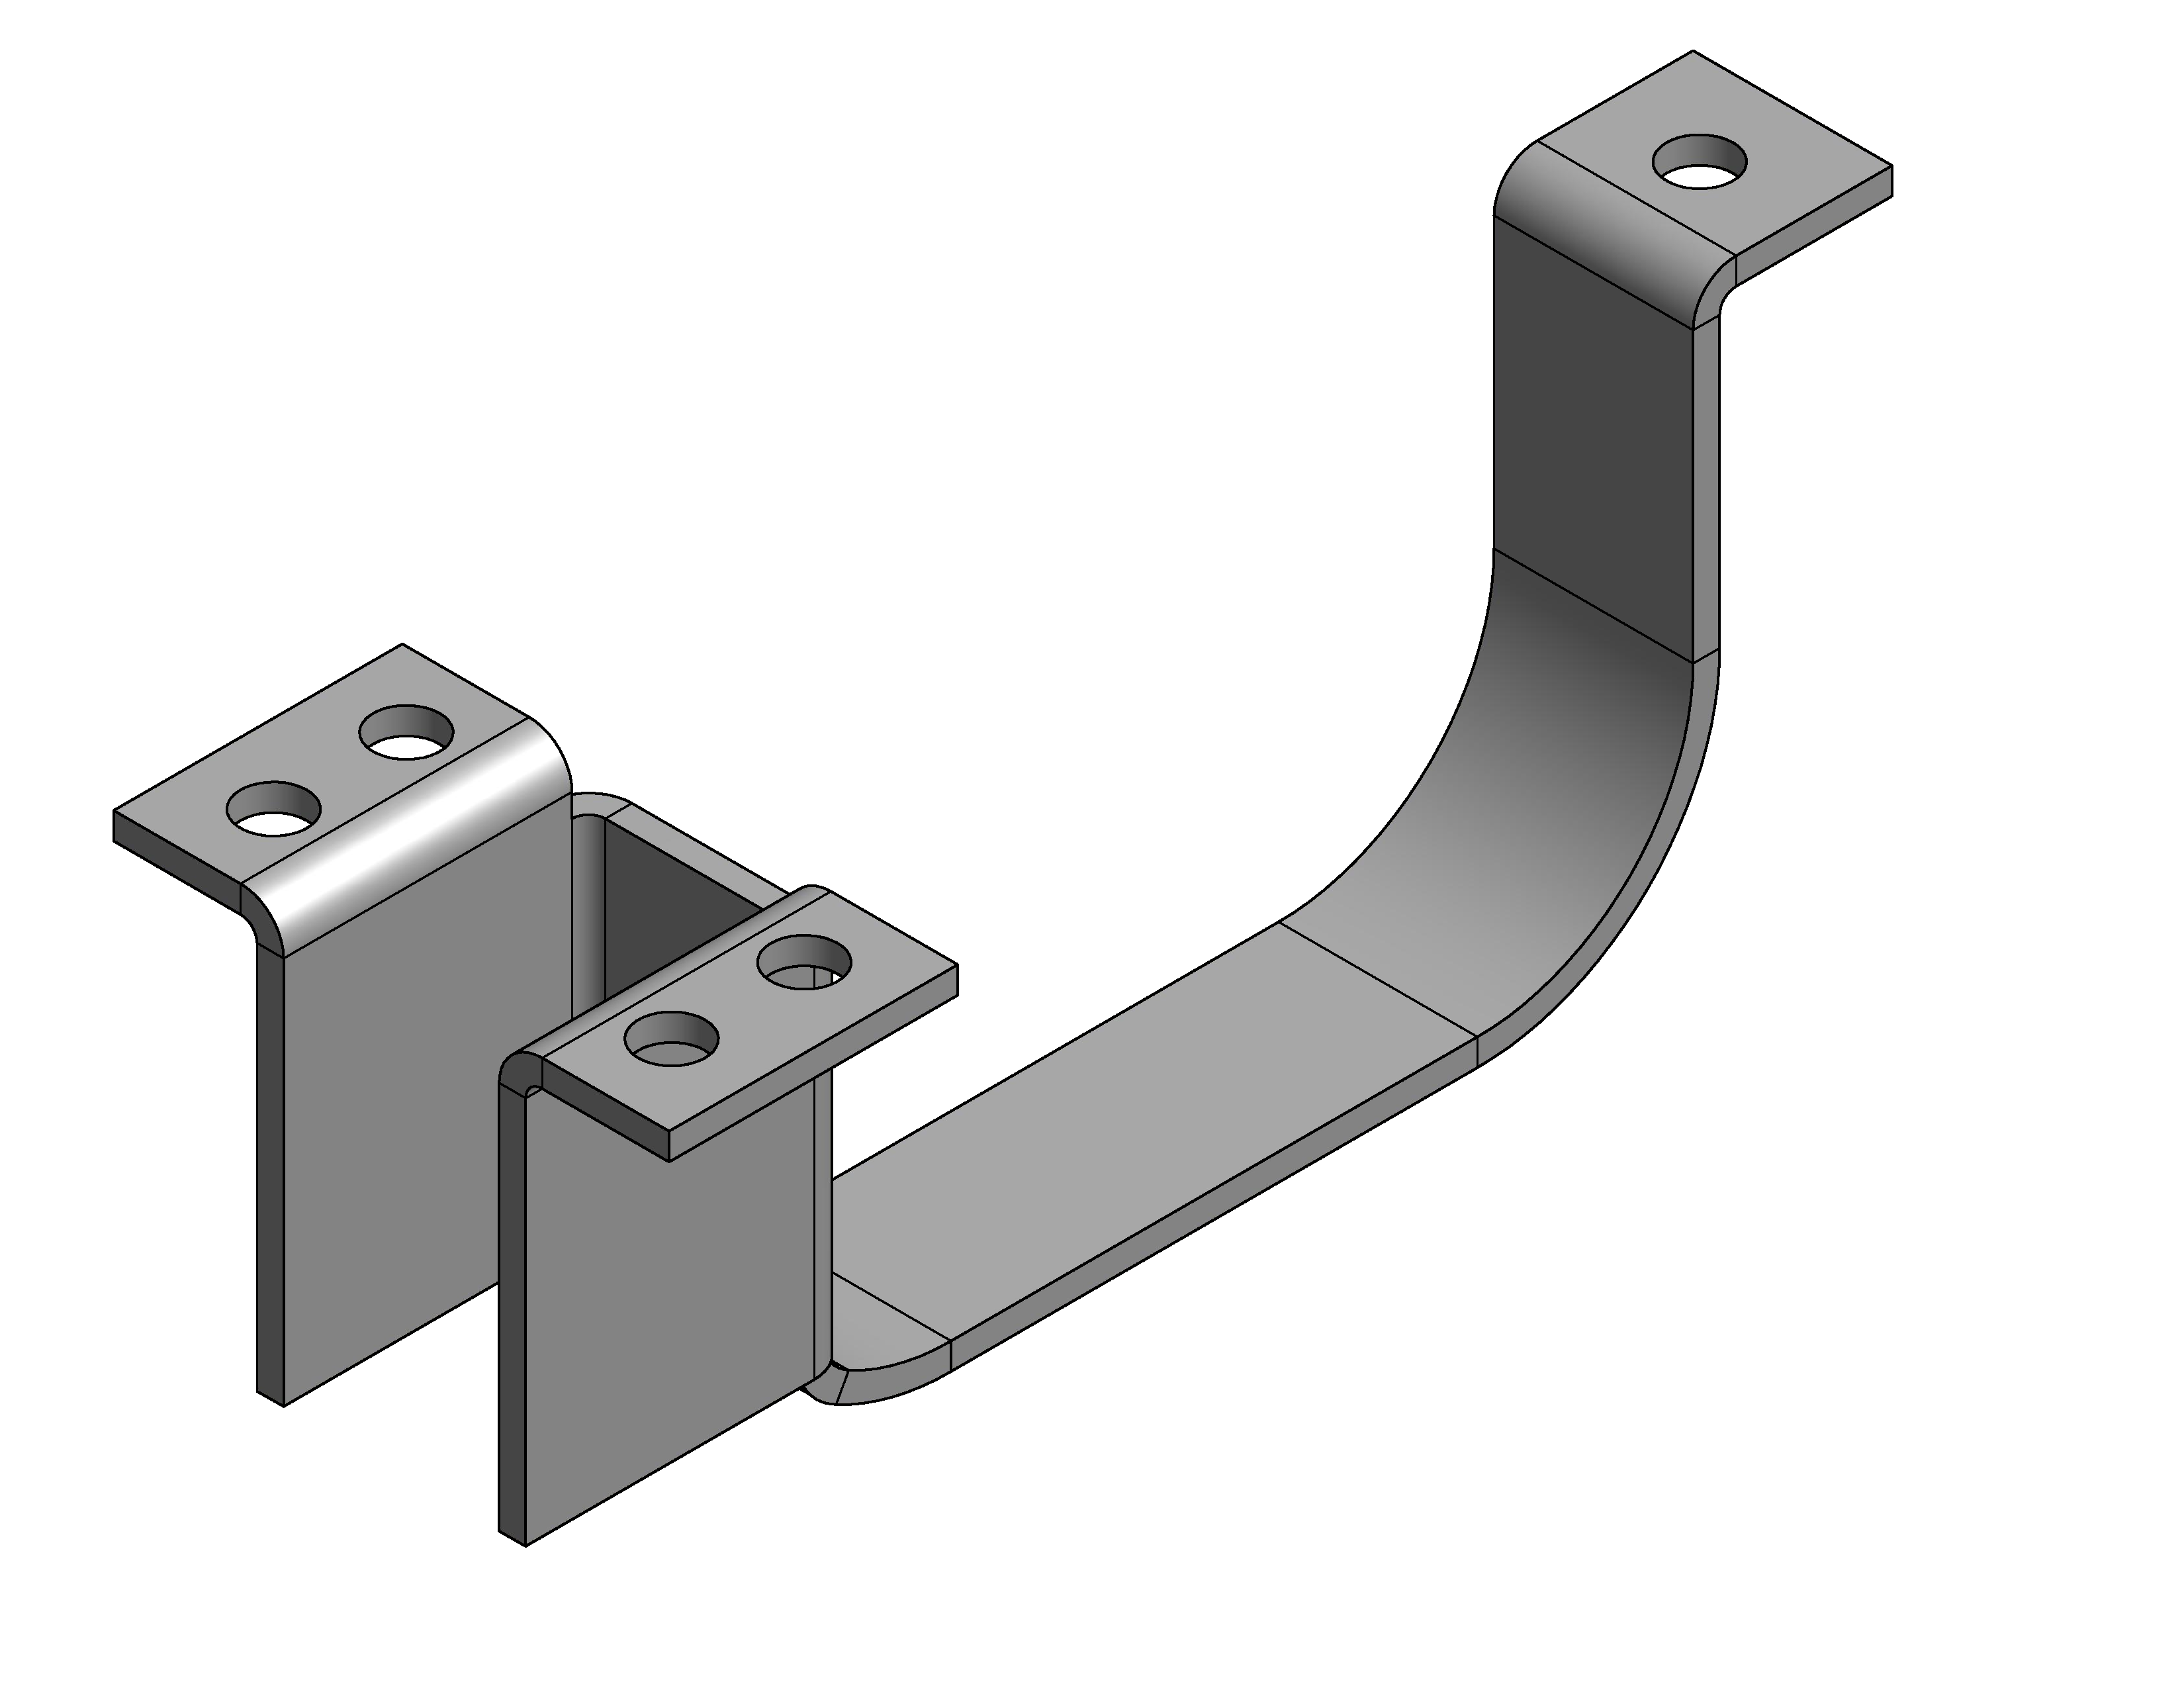
\includegraphics[width=0.43\linewidth]{images/SimpleBracketshaded.pdf}} \quad
\subfloat[Cellular Decomposition]{\label{fig_SimpleBracket_1}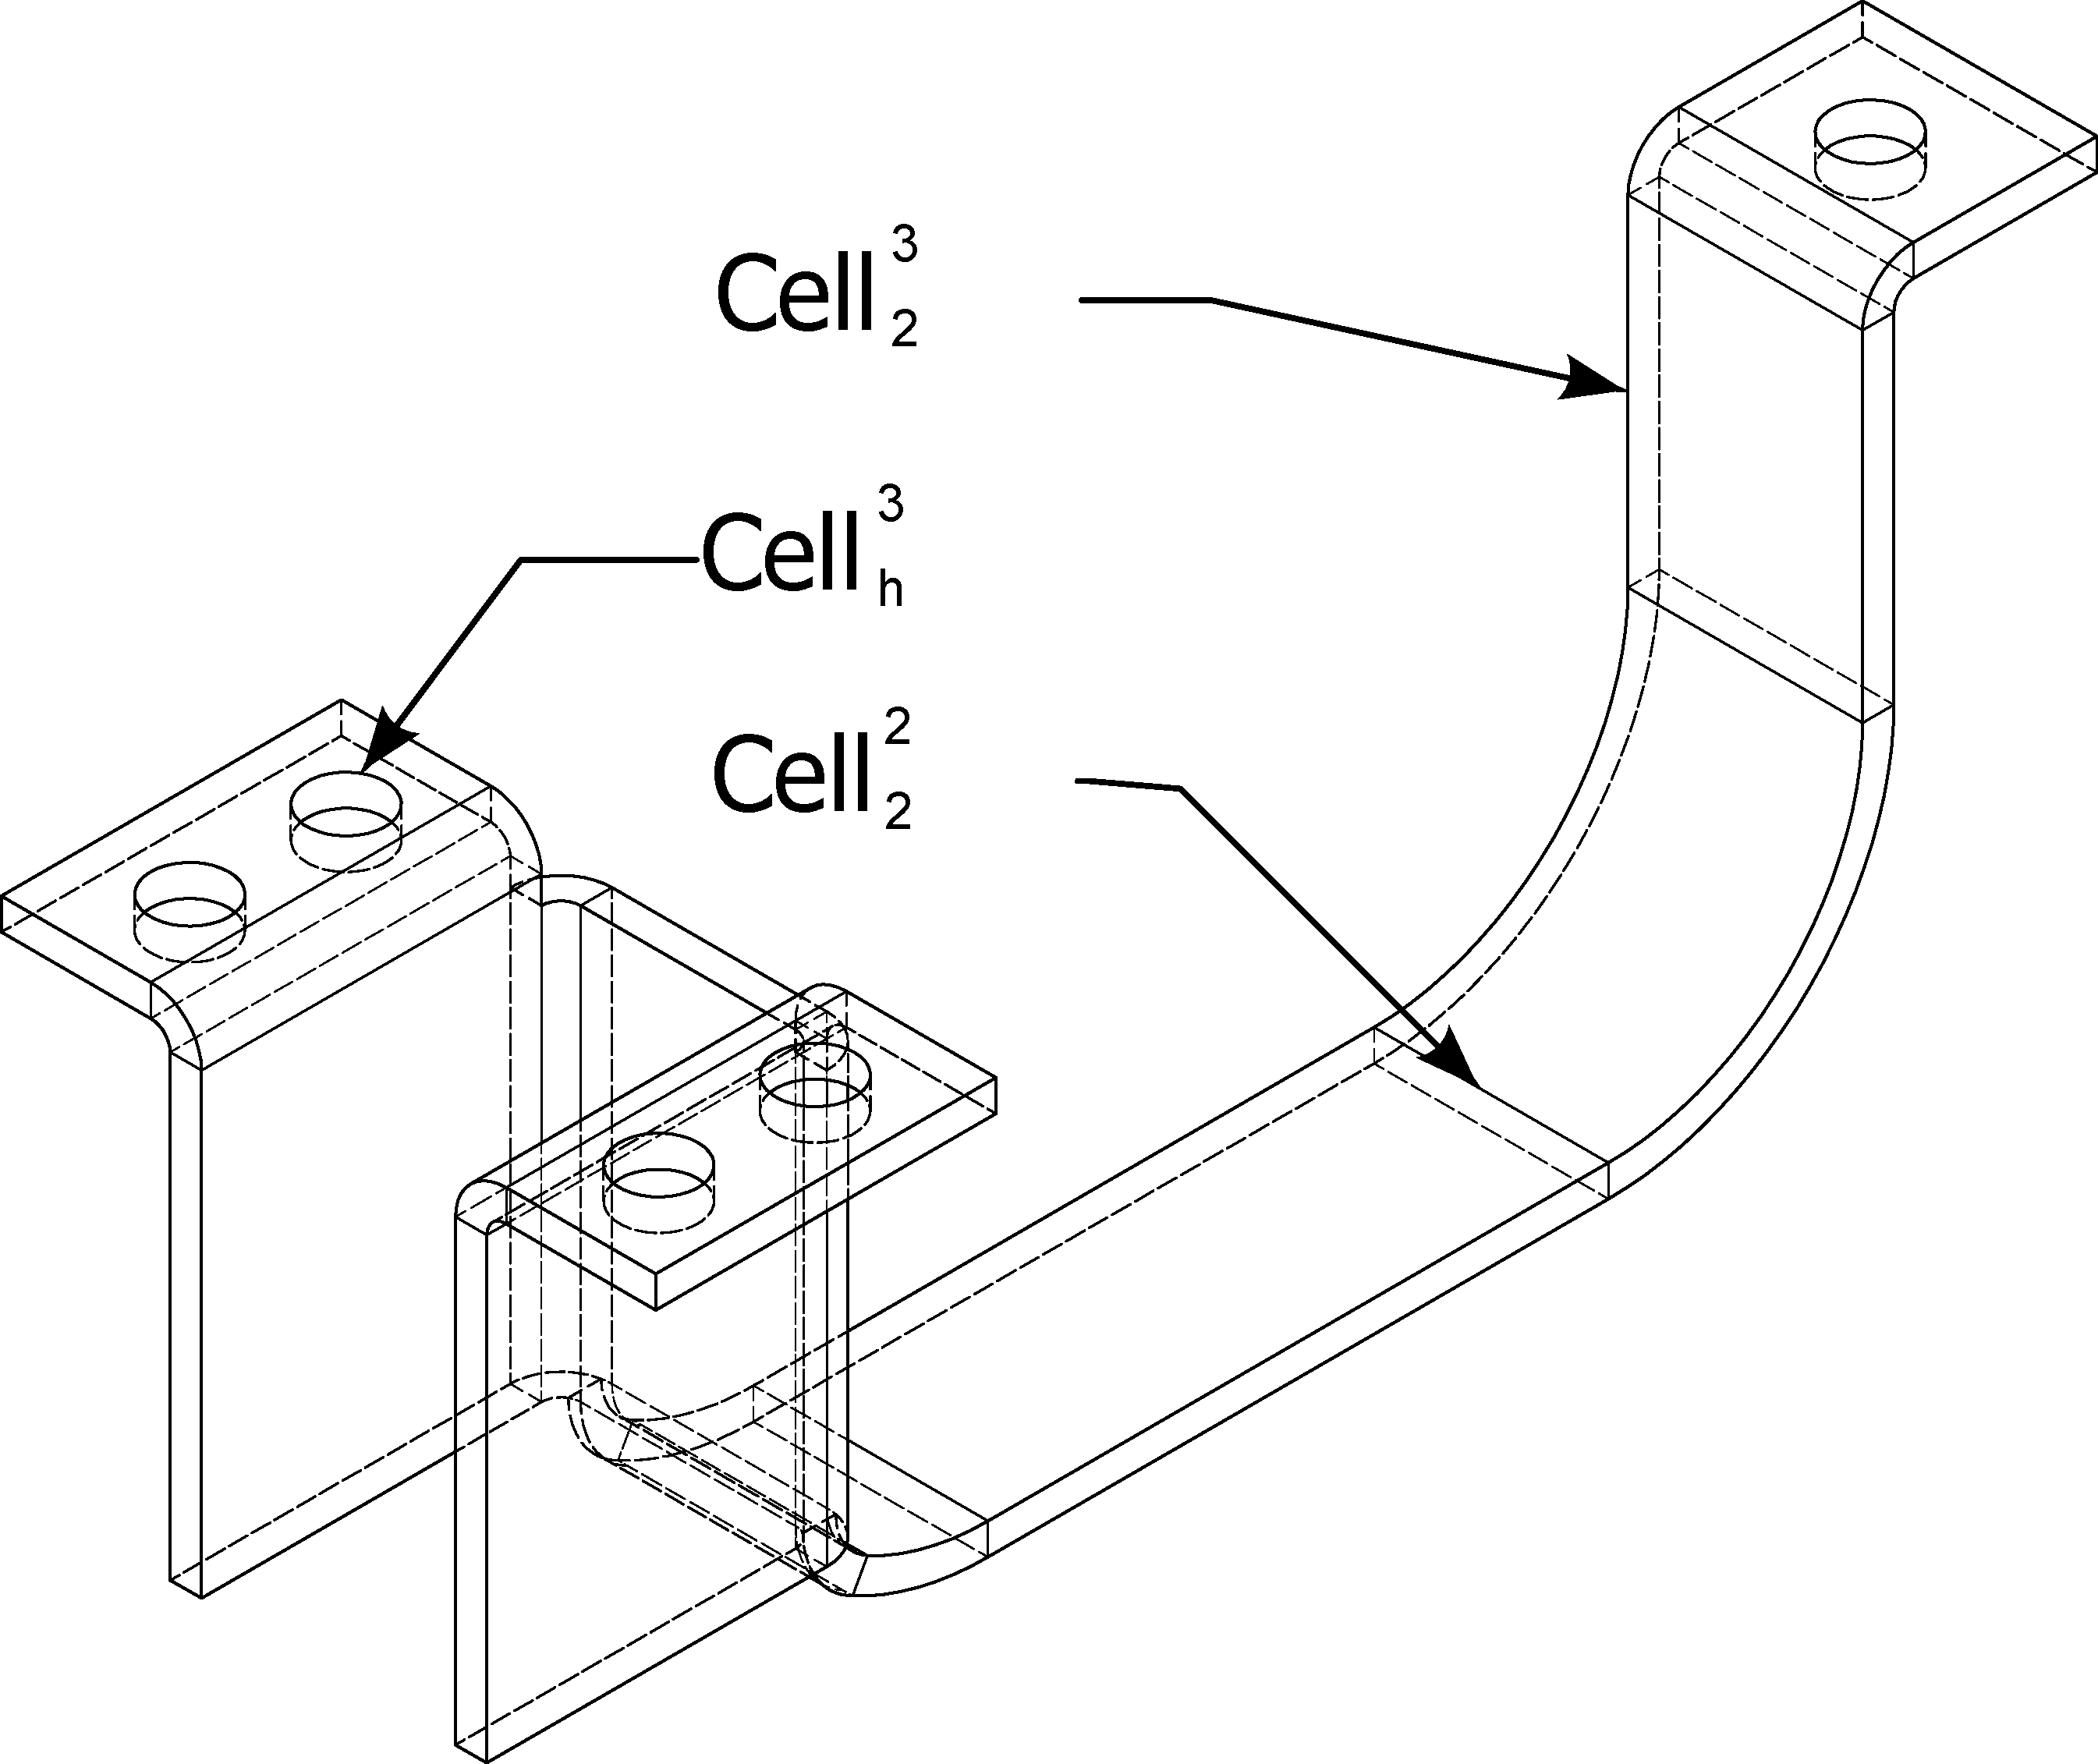
\includegraphics[width=0.43\linewidth]{images/SimpleBracket_1.pdf}} \quad
\caption{Solid to Surface Transformation Approach for Bracket}
  \label{fig:midsurfcelljoin:solidsurfbracket}
\end{figure}

%%\bigskip

Figure~\ref{fig_SimpleBracketshaded} shows the input solid whereas Figure~\ref{fig_SimpleBracket_1} shows the cellular topology. Steps listed below show formulations as per the equations derived before.

%\begin{tabular}[htp]{@{}p{0.48\linewidth}  p{0.48\linewidth}@{}} \toprule
%{\centering  \bf Solid} & { \centering  \bf Cellular Classification} \\ \midrule
%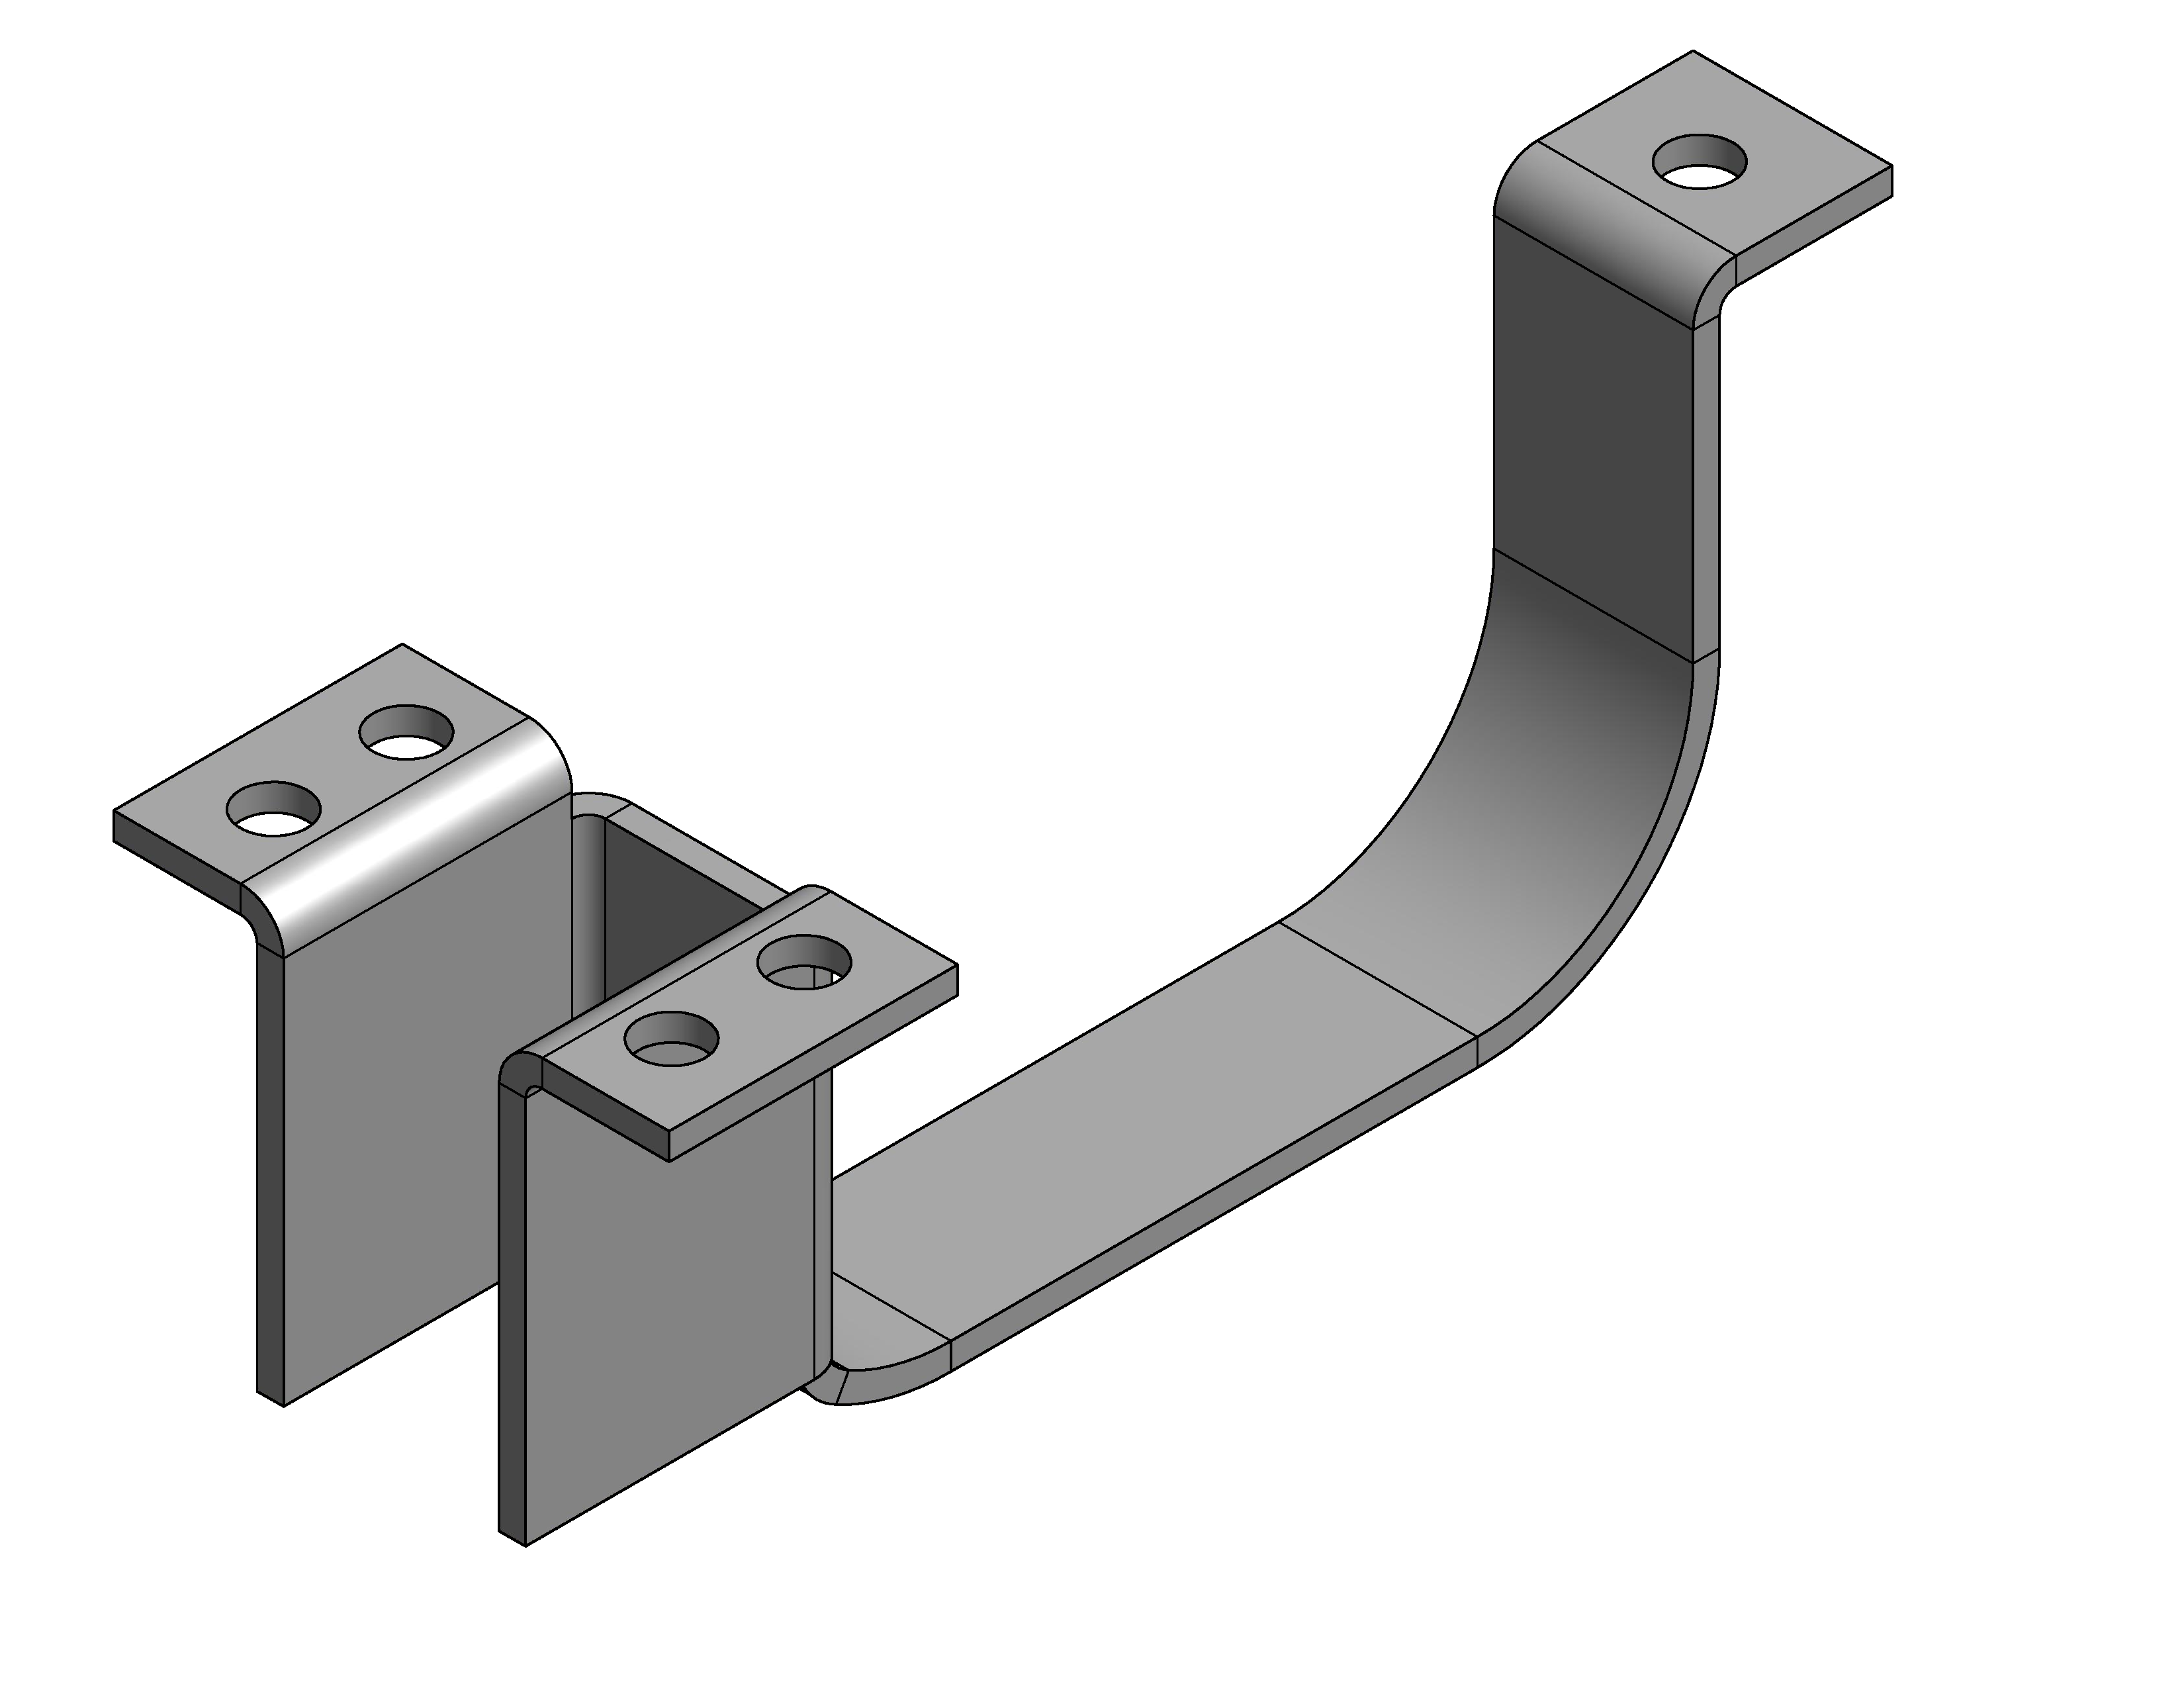
\includegraphics[width=\linewidth]{images/SimpleBracketshaded.pdf} &
%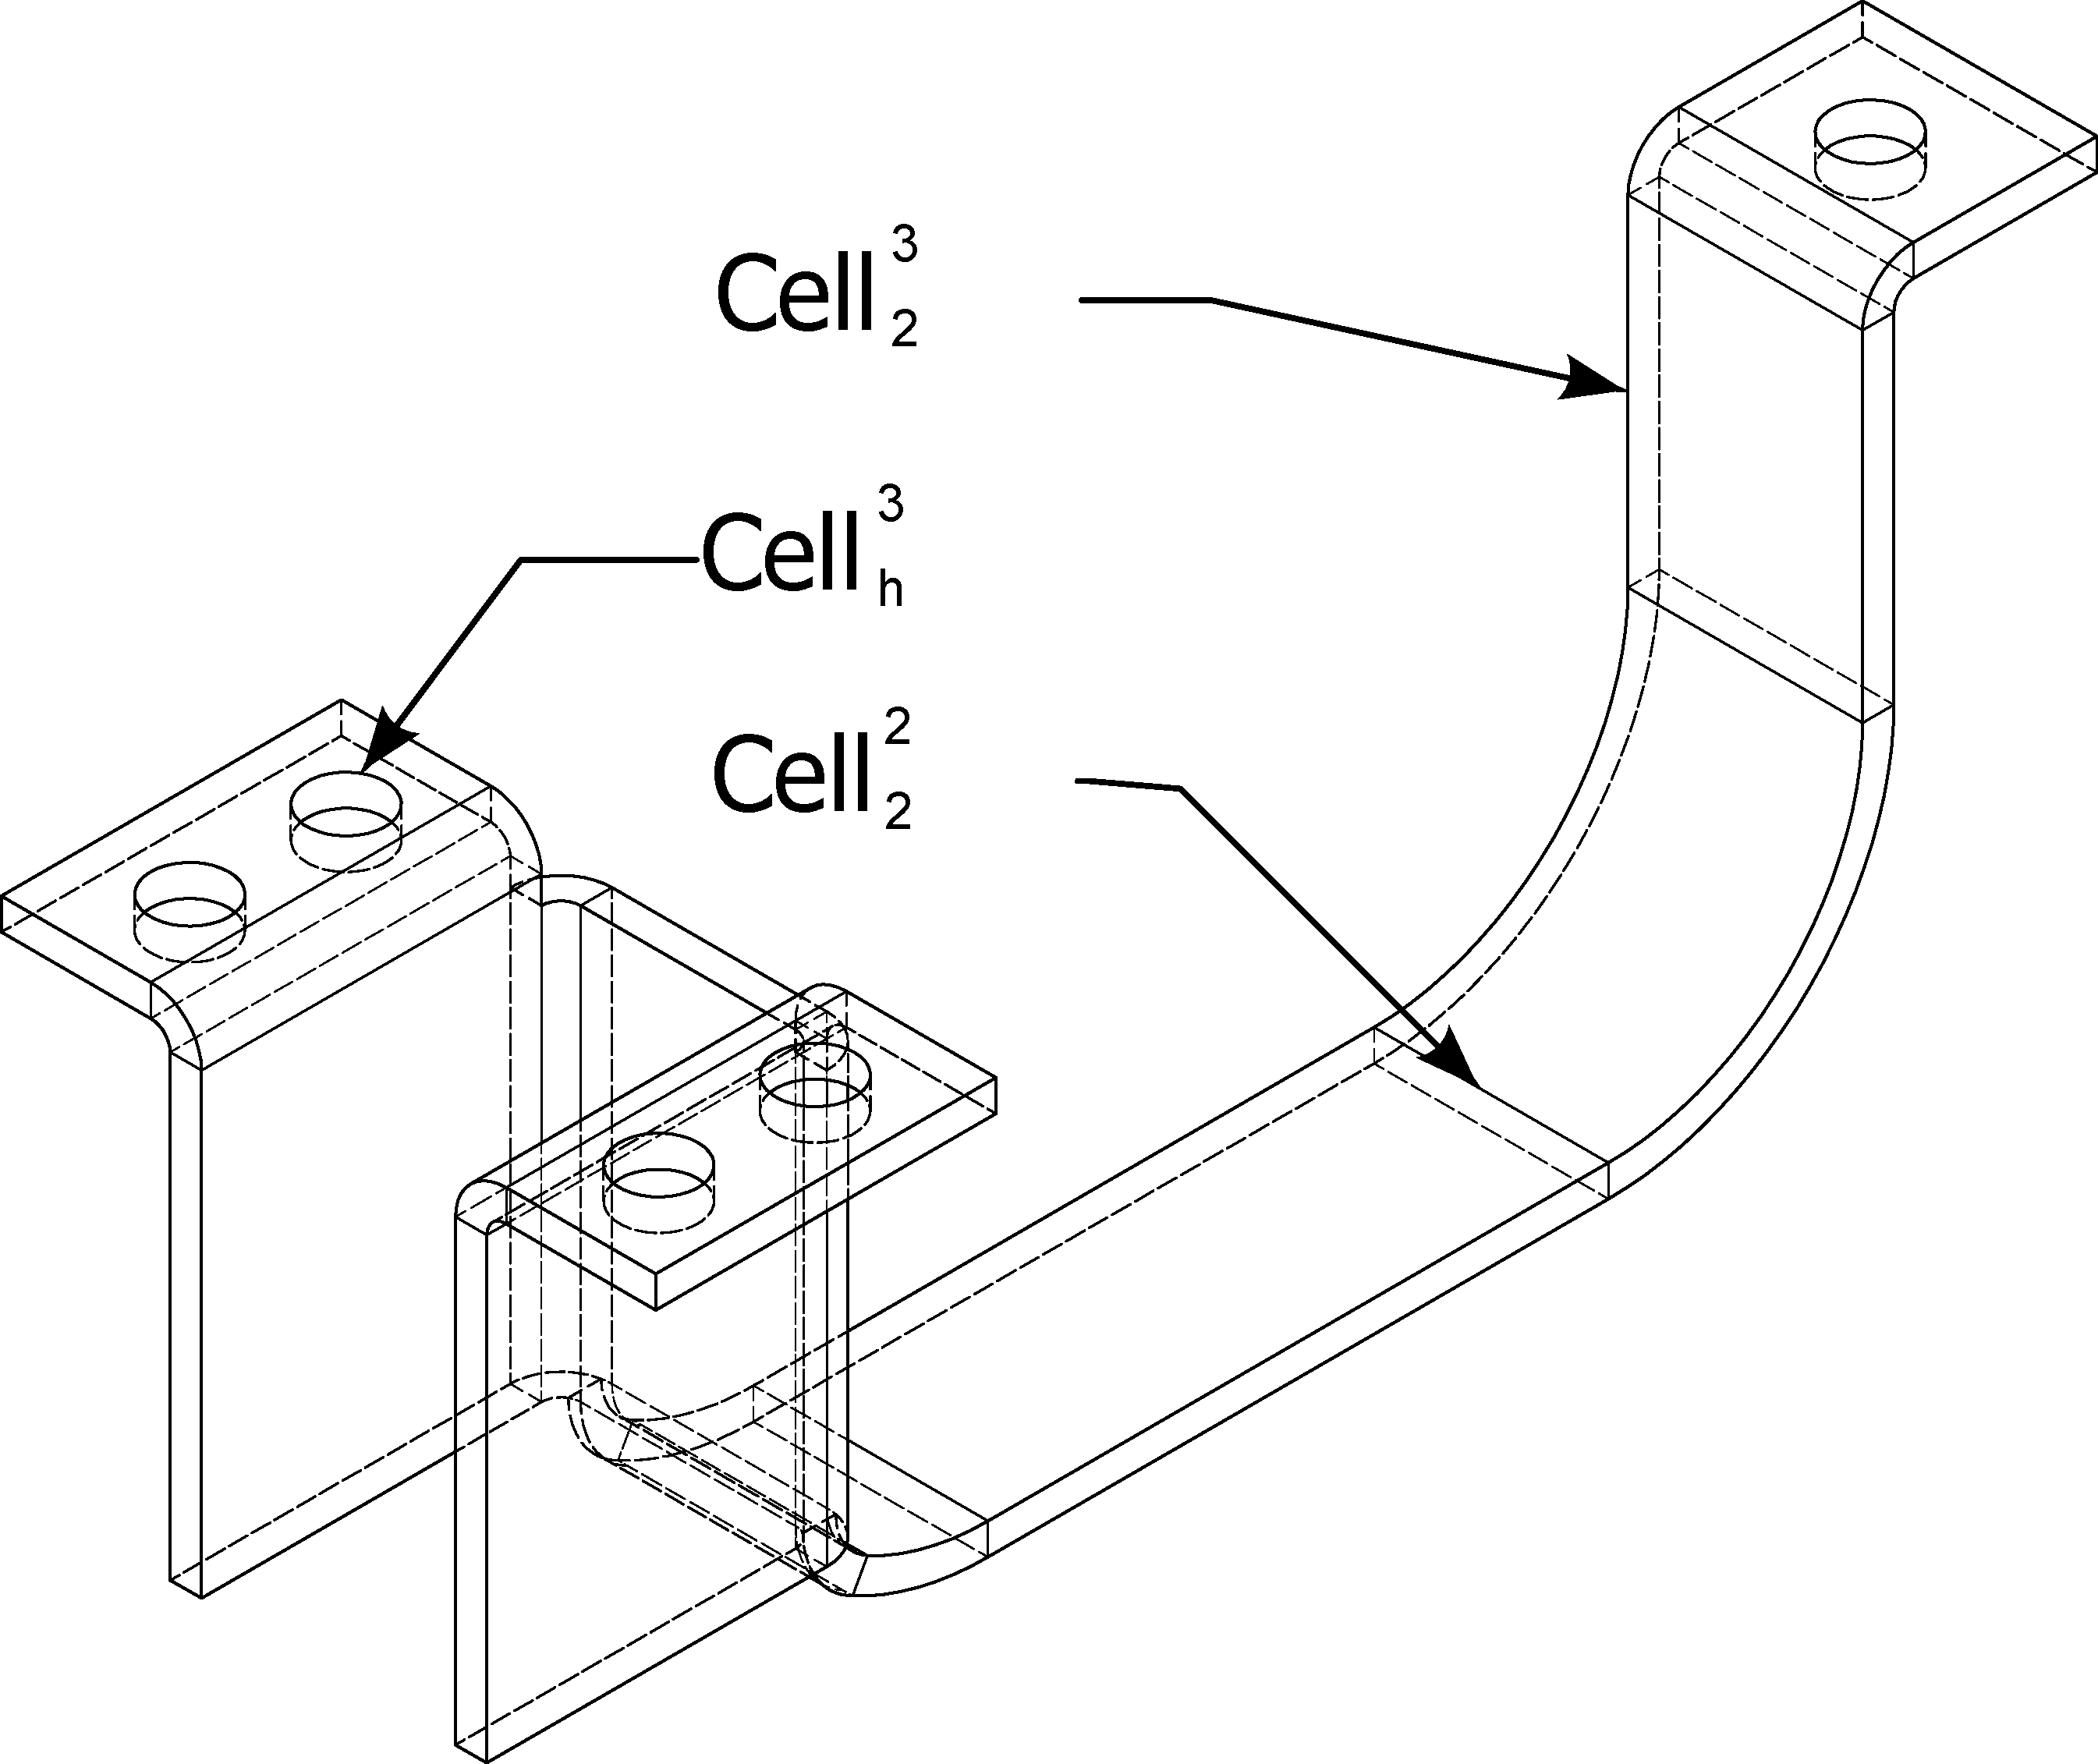
\includegraphics[width=\linewidth]{images/SimpleBracket_1.pdf}\\ \bottomrule
%\end{tabular}

\begin{itemize}
[noitemsep,topsep=2pt,parsep=2pt,partopsep=2pt,leftmargin=*]
	\item \textbf {Solid cells}: \newline  $5 \times sCell_{3,h} + 3 \times sCell^{3}_{1} + 13 \times sCell^{3}_{2} + 14 \times iCell^{2}_{2} $
	\item \textbf {Transformed Midsurface Cells}: \newline $5 \times mCell^{2}_{h} + 3 \times mCell_{2,1} + 13 \times mCell^{2}_{2} + 14 \times mCell^{1}_{2}$
	\item \textbf {Predicted midsurface Entities}:  \newline $5(1e+1v) + 3 (1f+3e+2v) + 13 (1f+2e+0v) + 14(1e+2v) = 
16f + 54e + 39v$
\end{itemize}


The derived formulation (Eqn   \ref{eqn:topoval:cellulara}, \ref{eqn:topoval:cellularaf}, \ref{eqn:topoval:cellularna}, \ref{eqn:topoval:cellularah} ) predicts correct topological entities for the midsurface. These, when substituted in the non-manifold equation (Eqn \ref{eqn:topoval:nonmanifold}) also prove to be valid. With $s=1, r=5, h=5$, the equation matches both sides:
$ 39 - 54 + (16 -5) = 1 (1-5)$

\todo{Review comment: Provide conclusion, summary, comment on contribution, comparision with others etc. [DONE]}.

Thus the above mentioned approach can be used to predict midsurface entities of an input solid. For validation, these predicted entities need to be compared with the topological entities of the actual midsurface. If they match, then topological validation is successful and then geometric validation can be carried out. If there is any mismatch, the errors need to investigated and fixed. Unlike the approach presented by Lockett~\cite{Lockett2008}, the proposed approach elaborated above, uses only topological entities and not the geometrical ones like angles, proximity groups, etc. as done in Lockett's work.

Following subsection presents the second sub-approach, that is of dimension-addition.

\subsection{Midsurface to Sheet Metal Solid Transformation} \label{sec:topoval:surfsolid}
In this approach, given a midsurface, topological entities  of its corresponding sheet metal solid are predicted. These predicted entities are verified to check if they match with the topological entities of the actual solid. Apart from this, the predicted entities are also validated against the manifold equation (Eqn \ref{eqn:topoval:manifold}). 

The proposed approach here uses additional classification of topological entities, that is typically available in Brep. These additionally classified entities are used to propose the dimension addition transformation. For example, vertices are classified as sharp, radial, internal, whereas edges are classified as sharp,cross-radial, side-radial, internal, etc. The proposed approach provides dimension addition of these entities as they get transformed into topological entities of the solid. \deleted{Topological entities of midsurface contains far richer (classifiable) topological information than its corresponding solid model.}

%%\bigskip

	\begin{figure}[!h]
	\centering     %%% not \center
	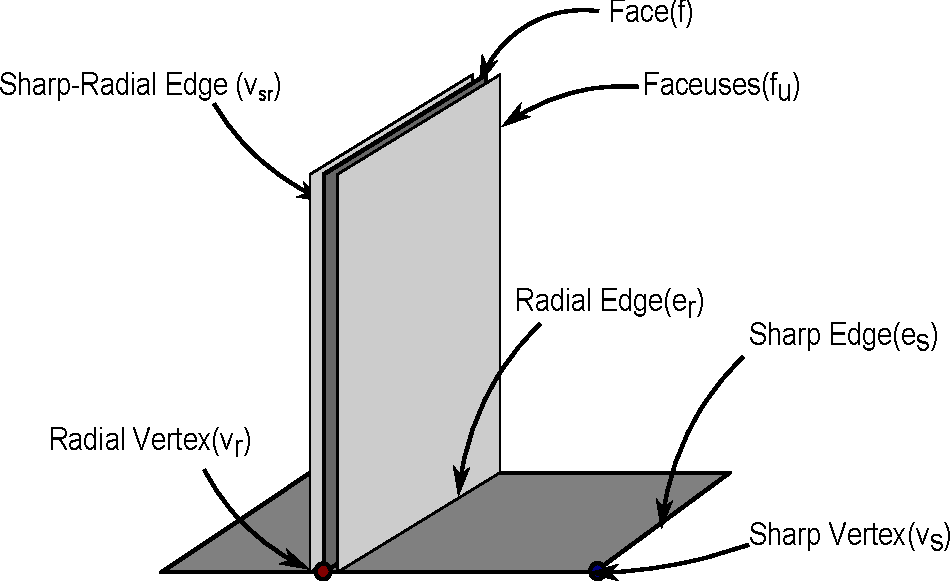
\includegraphics[width=0.62\linewidth]{images/NonManifoldT2.pdf}
	\caption{Non-Manifold Topological Entities}
	\label{fig:topoval:nonmanifold}
	\end{figure}

%%\bigskip


Figure~\ref{fig:topoval:nonmanifold} shows midsurface of ``T'' shaped solid, along with the classified topological entities. Apart from known topological entites, a few new ones have been defined and used in the approach, as below:

\begin{itemize} 
[noitemsep,topsep=2pt,parsep=2pt,partopsep=2pt,label=\textbullet]\label{lst:topoval:topos}
\item Face ($f$): A face is composed of two face-uses $f_u$. Face-uses are also known as Co-Faces or Half-Faces in other Brep terminologies~\cite{Hegde2013}.

\item Sharp Vertex ($v_s$): A vertex is a sharp vertex if it is connected to two edges of the same face.
\item Sharp Edge ($e_s$): An edge is a sharp edge if it is connected to two sharp vertices.

\item Radial Vertex ($v_{r}$): A vertex is a radial vertex if it is connected edges of different faces.
\item Degree ($n_{r}$) at the radial edge is the number of faces attached to it 
\item Cross Radial Edge ($e_{r}$): An edge is a cross radial edge if it is connected between two radial vertices and connects two different faces.
\item Side-Radial  Edge ($e_{rr}$): An edge is a side radial edge if it is connected between two radial vertices and is of same face
\item Sharp-Radial Edge ($e_{sr}$): An edge is a sharp radial edge if it is between sharp and radial vertex.
\item Internal Edge ($e_i$): An edge is an internal edge if it is part of the inner edge-loop or ring of the face.
\item Internal Vertex ($v_i$): A vertex is an internal vertex if it is connected to the internal edge.
\item Internal Loop ($r_i$): A loop is an inner loop if it is composed of internal edges and vertices.
\end{itemize}

%\begin{minipage}[t]{\linewidth}
%\centering 
%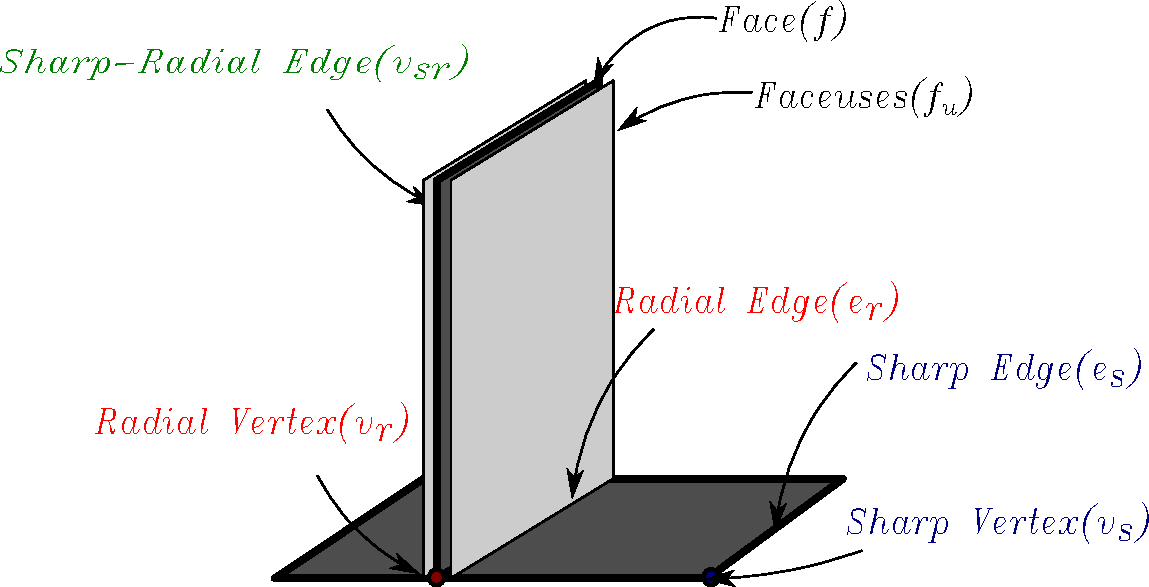
\includegraphics[width=0.6\linewidth]{images/NonManifoldT1.pdf}
%\vspace{2mm}
%\captionof{figure}{Non-Manifold topological entities}
%\label{fig:topoval:nonmanifold}
%\end{minipage}


	
Using the topological entities defined above, the dimension addition transformation is elaborated as follows.
%	
%\subsubsection{Steps: Topological Dimension Addition}
The basic principal of the approach is that a solid can be imagined to be a thickened midsurface. Each topological entity of the midsurface can be transformed to its higher-dimension counter part to create a solid. The solid will be of thin-walled type and will have thickness faces, called capping faces as well as non-thickness faces, called principal faces.


%%\bigskip

	\begin{figure}[!h]
	\centering     %%% not \center
	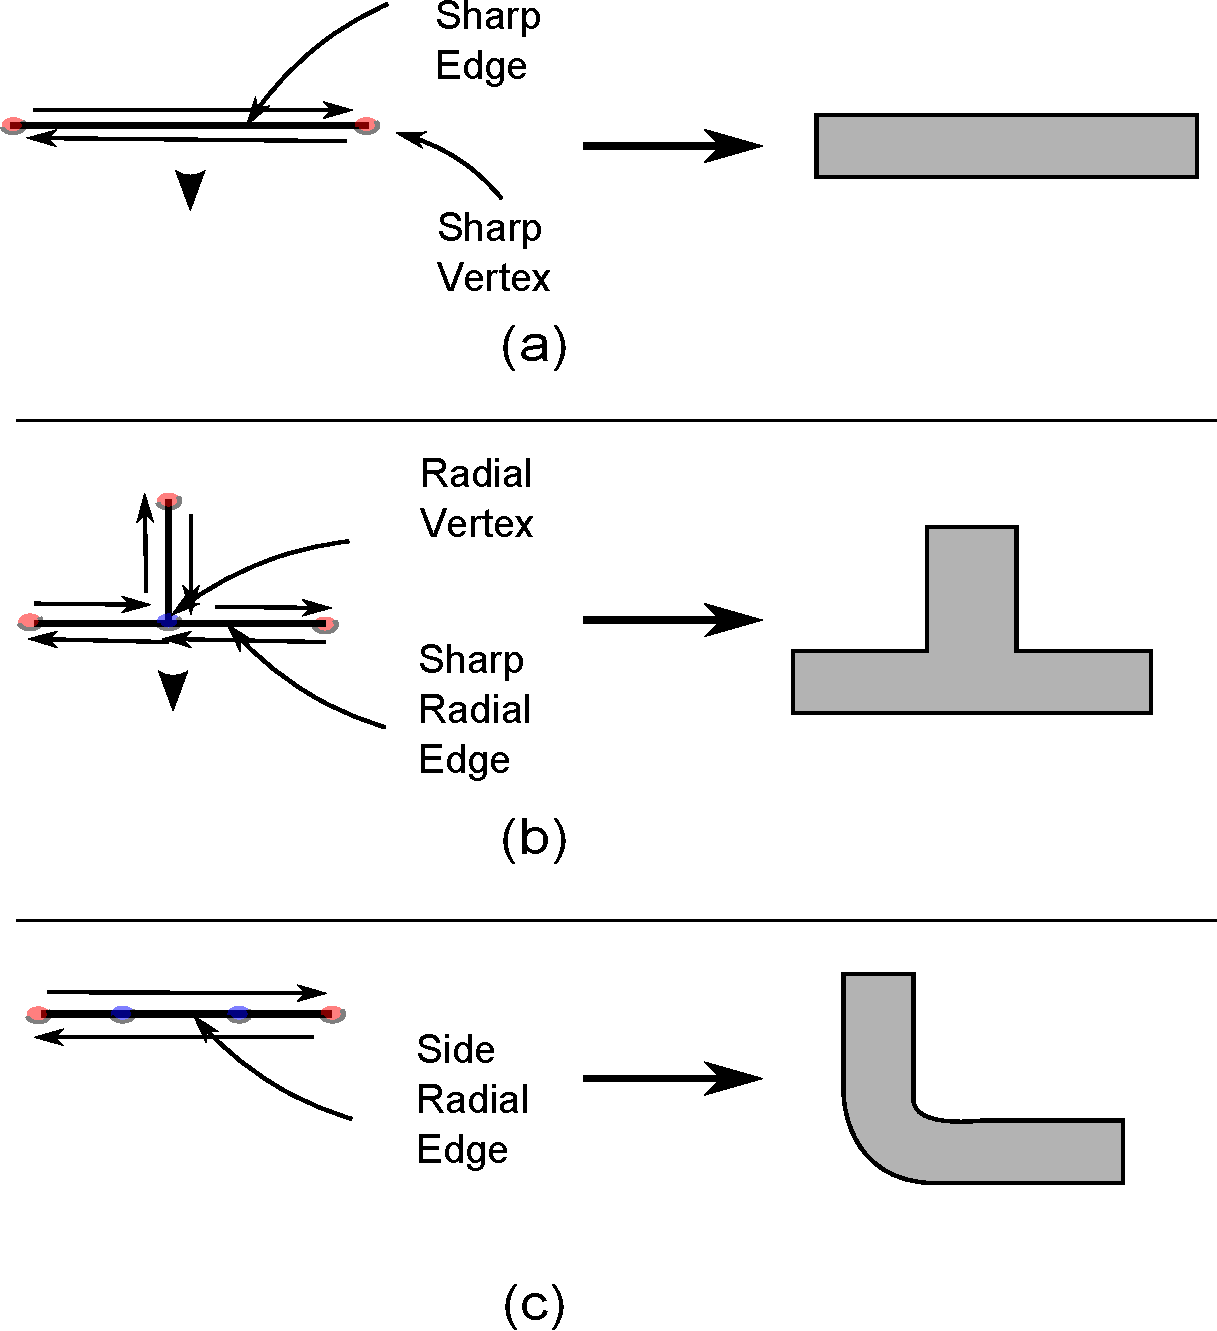
\includegraphics[width=0.62\linewidth]{images/NonManifoldLoopsToFaces2.pdf}
	\caption{Transformation of Loops from Midsurface to Faces of the Solid}
	\label{fig:topoval:loopstofaces}
	\end{figure}

%%\bigskip
	
Figure~\ref{fig:topoval:loopstofaces} shows some of the dimension addition transformations, from midsurface topological entities to solid topological entities. Figure~\ref{fig:topoval:loopstofaces}(a) shows that an edge on midsurface, which has got classified as a sharp edge, becomes a face in the solid.  Figure~\ref{fig:topoval:loopstofaces}(b) a ``T'' Shaped junction of edges, which have got classified as radial edges, along with a radial vertex, get transformed into a face in the solid.

The topological entities of the generated solid are transformed from midsurface entities as per following rules: %via relations in the Table \ref{table_TopoVal}.

\begin{itemize}
[noitemsep,topsep=2pt,parsep=2pt,partopsep=2pt,leftmargin=*]
\item Face-uses on the midsurface become principal faces in the solid.
 \item Sharp vertices on the midsurface become capping edges in the solid.
\item Apart from edge-use loop corresponding to face-use, a new loop is proposed for side-capping faces. The loop is formed between two sharp vertices ($v_s$) using  more than one sharp  ($e_{sr}$) or side radial ($e_{rr}$) edges but not using the cross radial edge ($e_r$). Such independent paths creating individual side faces are called $l_p$.
\item Loop between two sharp vertices. This gives rise to a singular capping face  (Fig.~\ref{fig:topoval:loopstofaces} a).
\item Loop between three branched sharp vertices. This gives rise to a combined capping face (Fig.~\ref{fig:topoval:loopstofaces}  b).
\item Loop between two sharp vertices with multiple radial vertices in between them. This gives rise to a combined capping face (Fig.~\ref{fig:topoval:loopstofaces}  c).
\end{itemize}
	
%
%\begin{minipage}[t]{\linewidth}
%\centering 
%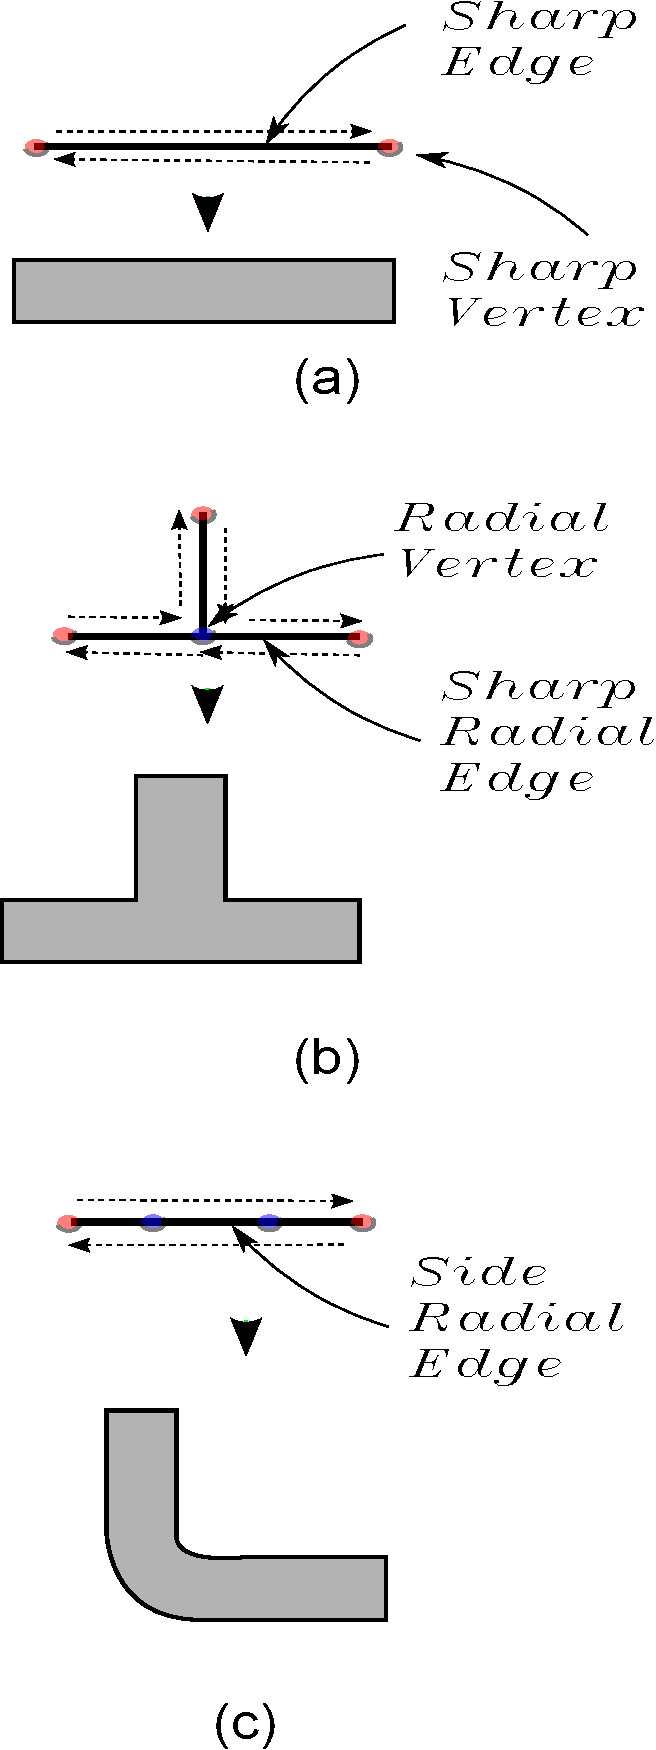
\includegraphics[width=0.225\linewidth]{images/NonManifoldLoopsToFaces1.pdf}
%
%\captionof{figure}{Loops to Faces}
%\label{fig:topoval:loopstofaces}
%\end{minipage}

\todo{Review comment: Is it your contribution? [YES. MENTIONED ``PROPOSED'']}

Based on the rules above, classified topological entities on the midsurface contribute to topological entities of the solid. Conversely, the topological entities of solid are made up of contribution from dimension addition of various topological entities on the midsurface. Thus, the proposed approach predicts topological entities in the solid with formulations as follows. The term ``manifold'' and the corresponding suffix $_m$,  are used for predicted entities of the solid. % (Summary in Table \ref{table_TopoVal}):

\begin{itemize}
[noitemsep,topsep=2pt,parsep=2pt,partopsep=2pt,label=\textbullet]
\item \textbf{Manifold-Vertices  ($v_m$)}: Number of vertices in the solid are calculated by doubling the number of sharp and internal vertices (one up  and  one below) + vertices for junctions which are denoted by the summation of  number of radial vertices times their corresponding degrees.
\begin{equation}
v_m = 2 (v_s + v_i) + \sum n_{r} v_{r} \label{eqn:topoval:vm}
\end{equation}
\item \textbf{Manifold-Edges ($e_m$)}: Number of edges in the solid are calculated by doubling the number of sharp, sharp-radial and internal edges (offset up and down) + degree times radial edges for offsets at junctions + sharp vertices for vertical-capping edges + internal vertices for vertical seam edges.
\begin{equation}
e_m = 2 (e_s + e_{sr} + + e_{rr} + e_i) + \sum n_r e_r  + v_s + v_i\label{eqn:topoval:em}
\end{equation}
\item \textbf{Manifold-Faces ($f_m$)}: Number of faces in the solid are calculated by doubling the number of faces (offset up and down) + sharp edges for capping faces + paths to have one combined face + internal edges for capping internal faces
\begin{equation}
f_m = 2f + e_s + l_p + e_i \label{eqn:topoval:fm}
\end{equation}
\item \textbf{Manifold-Shells ($s_m$)}: Number of shells remain the same in the solid.
\item \textbf{Manifold-Rings ($r_m$)}: Number of rings in the solid are calculated by doubling the number of internal rings on the midsurface.
\begin{equation}
r_m = 2r_i\label{eqn:topoval:rm}
\end{equation}
\item \textbf{Manifold-Genus ($h_m$)}: Number of Internal ring on midsurface become same number of holes (genus) in the solid.
\begin{equation}
h_m = r_i\label{eqn:topoval:hm}
\end{equation}
\end{itemize}

Once the manifold (i.e solid) topological entities are calculated, they can be verified by Euler-Poincar\'e Equation (Eqn~\ref{eqn:topoval:manifold}) by comparing left and right hand sides of the equations. Each side has to match to an invariant denoted as $\chi$.  Similarly input midsurface's verification can be done by Equation (Eqn~\ref{eqn:topoval:nonmanifold}).

With the above mentioned transformation rules, the proposed approach states procedure to validate the midsurface as below:

%\subsubsection{Procedure to Validate Midsurface}
\begin{enumerate}
\item The number of classified topological entities of the midsurface are counted as per the definitions suggested in Section~\ref{lst:topoval:topos} and shown in Figure~\ref{fig:topoval:nonmanifold}%such as $f, e_s , e_{sr} , e_{rr}, e_r , e_i, v_s , v_r , v_i, s , h , r$.
\item Based on dimension addition transformation equations \ref{eqn:topoval:vm}, \ref{eqn:topoval:em}, \ref{eqn:topoval:fm}, \ref{eqn:topoval:rm}, \ref{eqn:topoval:hm}, number of predicted topological entities of the corresponding input solid are calculated using equations, as follows:
	\begin{enumerate}
		\item Predicted number of manifold faces: $f_m \newline = 2f+e_s+ l_p +e_i $
		\item Predicted number of manifold edges: $e_m \newline = 2(e_s+e_{sr}+e_{rr}+e_i )+ \sum n_{r} e_{r}+v_s+v_i $
		\item Predicted number of manifold vertices: $v_m \newline= 2v_s+ \sum n_{r} v_r+2v_i$
		\item Predicted number of manifold shells, holes and rings: \newline$s_m =s = 1, h_m = r_i  = 0, r_m = 2r_i = 0$
	\end{enumerate}
\item Verify that the topological entities of the midsurface satisfy the non-manifold equation (Equation \ref{eqn:topoval:nonmanifold}), by deducing that the left ($\chi_{nml}$) and right  ($\chi_{nmr}$) hand side of the equation matches.
	\begin{enumerate}
		\item Input midsurface's non-manifold equation's left side  $\chi_{nml} \newline= v-e+f $
		\item Input midsurface's non-manifold equation's  right side  $\chi_{nmr} \newline=s-h+r$
%		\item Sheet metal midsurface characteristic $\chi_{smm} \\=
%		e_s+e_i+(2-n_{r} ) e_{r}+e_{sr}/n_{r} =v_s+(2-n_{r} ) v_{r}+v_i$
	\end{enumerate}
\item Verify that the predicted topological entities of the  thin-walled solid satisfy the manifold equation (Equation \ref{eqn:topoval:manifold}), by deducing that the left ($\chi_{ml}$) and right  ($\chi_{mr}$) hand side of the equation match; thus proving that the transformation equations are valid. 
	\begin{enumerate}
		\item Solid's manifold equation's left side  $\chi_{ml} \newline= v_m-e_m+f_m $
		\item Solid's manifold equation's right side  $\chi_{mr}\newline=2(s_m-h_m )+r_m$
%		\item Sheet metal midsurface characteristic $\chi_{smm} \\=
%		e_s+e_i+(2-n_{r} ) e_{r}+e_{sr}/n_{r} =v_s+(2-n_{r} ) v_{r}+v_i$
	\end{enumerate}
%Same validity can be shown using just the $\chi_{smm}$ characteristic, as below.
%\item Verify that  $\chi_{smm}$ characteristic equation (Equation \ref{eqn_nonmanifolddiff}) matches. 
\end{enumerate}




%\subsubsection{Examples}
Table \ref{tbl:topoval:simpleshapes2} displays the validation of midsurface using proposed dimension-addition-transformation equations. It is evident that the derived formulation works as the predicted entities validate the topological invariant $\chi_{m*}$ correctly. The validation is complete when these entities match with the actual solid's topological entities, and geometrical validation also assesses it positively.

%%\bigskip

\begin{minipage}{\linewidth}
\begin{center}
\captionof{table}{Validation of Midsurface (M)}
\label{tbl:topoval:simpleshapes2}
\begin{tabular}[t]{@{} p{0.1\linewidth}  
p{0.02\linewidth}  p{0.02\linewidth}  p{0.02\linewidth}   p{0.02\linewidth}  p{0.02\linewidth}  p{0.02\linewidth}     p{0.02\linewidth}  p{0.02\linewidth}  p{0.02\linewidth} p{0.02\linewidth}  p{0.02\linewidth}  p{0.02\linewidth}  p{0.02\linewidth}   p{0.02\linewidth}  p{0.12\linewidth}@{}} \toprule
{\bf M} & 
{\bf $f$}  		& {\bf $l_p$ } 	& {\bf $e_s$ }  	& {\bf $e_{sr}$} & {\bf $e_r$}  & 
{\bf $e_{rr}$} 	& {\bf $e_i$ } 	& {\bf $v_s$ } 	& {\bf $v_r$}  	&  {\bf $v_i$}  & 
{\bf $f_{m}$} 	& {\bf $e_m$ } 	& {\bf $v_m$ } 	& {\bf $\chi_{m*}$ } & {\bf Solid}  \\ \midrule 

\adjustbox{valign=c}{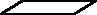
\includegraphics[width=\linewidth]{images/SimplePlane1.pdf}}  &  
1 & 0 & 4 & 0 & 0 & 0 & 0  & 4 & 0 & 0 & 6 & 12 & 8 & 2 
& \adjustbox{valign=c}{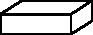
\includegraphics[width=\linewidth]{images/SimplePlate1.pdf}} \\ 

\adjustbox{valign=t}{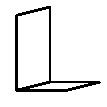
\includegraphics[width=\linewidth]{images/LPlane1.pdf}}  &  
2 & 2 & 2 & 4 & 1 & 0 & 0  & 4 & 2 & 0 & 8 & 18 & 12 & 2 
& \adjustbox{valign=c}{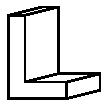
\includegraphics[width=\linewidth]{images/LPlate1.pdf}}  \\ 


\adjustbox{valign=t}{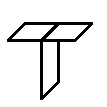
\includegraphics[width=\linewidth]{images/TPlane1.pdf}}  &  
3 & 2 & 3 & 6 & 1 & 0 & 0  & 6 & 2 & 0 & 11 & 27 & 18 & 2 
& \adjustbox{valign=c}{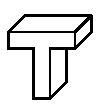
\includegraphics[width=\linewidth]{images/TPlate1.pdf}}  \\ 

\adjustbox{valign=c}{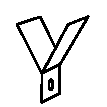
\includegraphics[width=\linewidth]{images/YwithHolem1.pdf}}  &  
3 & 2 & 3 & 6 & 1 & 0 & 1  & 6 & 2 & 1 & 12  &  30  & 20  & 2 
& \adjustbox{valign=c}{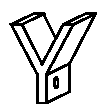
\includegraphics[width=\linewidth]{images/YwithHole1.pdf}} \\ 

\adjustbox{valign=c}{\includegraphics[width=\linewidth]{images/LwithRoundm1.pdf}}  &  
3 & 2 & 2 & 4 & 2 & 2 & 0  & 4 & 4 & 0 & 10  & 24  & 16  & 2 
& \adjustbox{valign=c}{\includegraphics[width=\linewidth]{images/LwithRound1.pdf}}  \\  
\bottomrule
\end{tabular}


\end{center}
\end{minipage}

%%\bigskip

%%\vspace{1mm}
%\subsection{Geometric Validation} \label{sec:topoval:geom}

\todo{Review comment: Where is the geometric validation'? [IT HAS NOT BEEN ADDED BECAUSE IT IS NOT THE CONTRIBUTION]}
%\section{Example}

\begin{figure}[h!]
\centering     %%% not \center
\subfloat[Input Midsurface]{\label{fig_SimpleBracketMidsurfshaded}\includegraphics[width=0.43\linewidth]{images/SimpleBracketMidsurfshaded.pdf}} \quad
\subfloat[Topological Entities Classification]{\label{fig_SimpleBracketMidsurf}\includegraphics[width=0.43\linewidth]{images/SimpleBracketMidsurf.pdf}} \quad
\caption{Solid to Surface Transformation Approach for Bracket}
  \label{fig:midsurfcelljoin:surfsolidbracket}
\end{figure}

Figure~\ref{fig_SimpleBracketMidsurfshaded} shows the midsurface of a sheet metal bracket's solid model, whereas Figure~\ref{fig_SimpleBracketMidsurf} shows classified topological entities of the midsurface. 

%%\bigskip



%%\bigskip


Steps listed below show formulations as per the equations derived before.

%\begin{tabular}[htp]{@{}p{0.48\linewidth}  p{0.48\linewidth}@{}} \toprule
%{\bf Midsurface} & {\bf Entities Classification} \\ \midrule
%\includegraphics[width=\linewidth]{images/SimpleBracketMidsurfshaded.pdf} &
%\includegraphics[width=\linewidth]{images/SimpleBracketMidsurf.pdf}\\ \bottomrule
%\end{tabular}

\begin{enumerate}
[noitemsep,topsep=2pt,parsep=2pt,partopsep=2pt,label=\textbullet]
\item \textbf{Midsurface entities}: \\$f = 15, e_s = 3, e_{sr} = 10, e_r = 14, e_{rr} = 19, l_p = 9 ,e_i=5,v_s = 8,v_r =24, v_i= 5, s=1,h=5,r=5$
\item \textbf{Predicted number of manifold-faces}: \\$f_m = 2f+e_s+ l_p +e_i $\\$= 2 \times 15 + 3 + 9 + 5 = 47$
\item \textbf{Predicted number of manifold-edges}: \\ $e_m = 2(e_s+e_{sr}+e_{rr}+e_i )+ \sum n_{r} e_{r}+v_s+v_i $\\$= 2(3+10+19 + 5)+ (2\times 12 + 4 \times 2)+8+5 = 119$
\item \textbf{Predicted number of manifold-vertices}: \\$v_m = 2(v_s+ v_i) + \sum n_{r} v_r$\\$=2\times (8 + 5)  + 2 \times 24=74$
\item \textbf{Predicted number of manifold-shells-holes}: \\$s_m =s = 1, h_m = r_i  = 5, r_m = 2r_i = 10$
\item \textbf{Input midsurface's non-manifold equation's left side}:  $\chi_{nml} $\\$= v-e+f $\\$= 32-46+15 = 1$
\item \textbf{Input midsurface's non-manifold equation's right side}:  $\chi_{nmr}$\\$=s-h+r$\\$=1-5+5 = 1$
\item \textbf{Solid's manifold equation's left side}:  $\chi_{ml} $\\$= v_m-e_m+f_m $\\$=74-119+47= 2$
\item \textbf{Solid's manifold equation's right side}:  $\chi_{mr}$\\$=2(s_m-h_m )+r_m$\\$= 2(1-5)+10 = 2$
%\item Sheet metal midsurface characteristic $\chi_{smm}$\\$=
%e_s+e_i+(2-n_{r} ) e_{r}+e_{sr}/n_{r} $\\$=v_s+(2-n_{r} ) v_{r}+v_i$\\$ 4+0+0+0=4+0+0= 4$
%\item \textbf{Result}: \textcolor{green}{Matches}
\end{enumerate}
It can be observed that the predicted solid entities validate the manifold equation ($\chi_{ml} = \chi_{mr} = 2$). Validation can also be performed by comparing the  topological entities of the thin-walled solid with the predicted ones.
